% Copyright 2018-2020 Jarred Vardy, ImmortalPharaoh7, Bryce AS202313, Lenart Bucar
\documentclass[a4paper, 12pt]{article}
%Paragraph jumps and indentation
\setlength{\parskip}{1.6em}
\setlength{\parindent}{1.25cm}
%Border
\usepackage[left=1in, right=1in, top=1in, bottom=1in]{geometry}
%Double spacing
\usepackage{setspace}
\doublespacing
%Indentation
\setlength{\parindent}{0pt}
%Bibliography
\usepackage{biblatex}
\addbibresource{references.bib}
%Packages
\usepackage{amsmath}
\usepackage[dvipsnames]{xcolor}
\usepackage{mathtools}
\usepackage{amsfonts}
\usepackage{titlesec}
%Images
\usepackage{graphicx}
\graphicspath{ {./images/} }
\usepackage{wrapfig}
\usepackage{float}
%SVGs
\usepackage{svg}
% Redefine the figure environment to automatically add [H] and vertical space
\let\oldfigure\figure
\let\endoldfigure\endfigure
\renewenvironment{figure}[1][H] % Default to [H] placement
  {\oldfigure[#1]\vspace{0.5cm}\centering} % Add vspace before the figure and center it
  {\endoldfigure\vspace{0.5cm}} % Add vspace after the figure
\let\oldtable\table
\let\endoldtable\endtable
\renewenvironment{table}[1][h]
  {\oldtable[#1]\vspace{0.5cm}\centering} % Add vspace before the figure and center it
  {\endoldtable\vspace{0.5cm}} % Add vspace after the figure
%Tables
\usepackage{multirow}
\usepackage{array}
\usepackage{tabu}
\titleformat{\section}
{\normalfont\large\bfseries}{\thesection}{1em}{}
\titleformat{\subsection}
{\normalfont\large\bfseries}{\thesubsection}{1em}{}
\usepackage{booktabs}
\usepackage{subcaption}
\counterwithin{equation}{section}
\usepackage{hyperref}
\urlstyle{same}
%Math Equation Size
\DeclareMathSizes{12}{12}{12}{12}
% Figure Caption Size
\usepackage{caption}
\captionsetup{font=small}
% Python Code Highlight
\usepackage{minted}
\newminted{python}{
  frame=lines,
  framesep=2mm,
  baselinestretch=1.2,
  fontsize=\footnotesize,
  linenos,
  breaklines
}
%Hyperlinks
\hypersetup{
    colorlinks=true,
    linkcolor=blue,
    filecolor=magenta,
    urlcolor=blue
}
% =========================================
%             DOCUMENT
% =========================================

\begin{document}

% =========================
%      TITLE PAGE
% =========================

\begin{titlepage}
    \begin{center}
        \vspace*{1cm}
        \large{\textbf{Computer Science}}\\
        \vspace{3cm}
        \Large{\textbf{Investigating Histograms of Oriented Gradients in Pedestrian Detection}}\\
        \vspace{1.5cm}
        \large{How does the sliding window size, block density, and the derivative mask of a Histogram of Oriented Gradients descriptor impact the performance of a linear Support Vector Machine pedestrian classifier?}\\
        \vspace{3cm}
        \large{Word Count: 2000}
        \vfill
        \large{May 2025}
    \end{center}
\end{titlepage}


% =========================
%      DOCUMENT BODY
% =========================

\pagenumbering{roman}

\begin{center}
\pdfbookmark{\contentsname}{Contents}
\tableofcontents
\vspace{1in}
\end{center}
\newpage
\pagenumbering{arabic}
\section{Introduction}\label{sec:introduction}
Pedestrian detection is a critical area of research in computer vision and artificial intelligence, with it being one of the extensively studied fields in the past decade \cite{dollar_2012_pedestrian}. The applications of automatic pedestrian detection span autonomous vehicles, surveillance systems, and robotics \cite{dollar_2012_pedestrian}. Most notably, automatically detecting pedestrians from moving vehicles could considerable impact economic and social welfare by substantially reducing pedestrian injuries and fatalities, which, in the European Union, make up 20\% of all road accidents \cite{slootmans_2021_european}

Pedestrian detection involves identifying and locating human figures in images or video frames, which presents unique challenges due to the variability in occlusions, diverse backgrounds and changing environmental conditions \cite{dollar_2012_pedestrian}. Alongside the many variables present in natural pedestrian environments, noise can arise during the image acquisition process, mainly due to imperfect instruments \cite{faraji_2006_ccd}. Therefore cleanly discriminating human appearance and the wide range of poses they can adopt calls for the use of a feature set which would be able to characterise object shape and orientation locally, so that changes in “noisy” regions (like an image’s background) do not significantly impact the feature detection in other regions that still provide useful information (like a pedestrian’s silhouette).

Histograms of Oriented Gradients (HOG) \cite{dalal_2005_histograms} is well-known \cite{dollar_2012_pedestrian} image processing algorithms because it solves the problem of variability and noise in pedestrian images by detecting one of the most essential features of images - edges \cite{niebles2012edge} \cite{dalal_2005_histograms}. Despite the suggested superiority of HOG \cite{dalal_2005_histograms} and widespread adoption in modern pedestrian classifiers \cite{dollar_2012_pedestrian}, the parameters used for the algorithm have remained essentially unchanged since the introduction of the method in 2005 \cite{dalal_2005_histograms}

Given the importance of the HOG descriptor in real life applications and significant improvements in the variety, difficulty and scale of pedestrian datasets since 2005 \cite{dollar_2012_pedestrian}, this investigation seeks to maximize the accuracy and performance of a linear Support Vector Machine (SVM) in pedestrian classification by varying the various properties of HOG.
\section{Background Information}
\subsection{Histograms of Oriented Gradients}\label{sec:hog}
The most prominent discriminative feature of pedestrians is their shape: limbs, head, and any features with prominent edges \cite{dalal_2005_histograms}. In that regard, HOG features are excellent at pedestrian detection precisely because they prioritize orientation/shape information, unlike other feature descriptors like HaaR wavelets which are colloquially described as “texture features” 
\cite{zia_2015_why}. 
\subsubsection{One Fundamental Property of Images}
At their core, images are matrices that represent pixel intensity values. 
Elements in grayscale image matrices contain a single intensity value, while elements in colored image matrices contain three (one for each color channel). With this definition of an image, it becomes increasingly simple to understand the meaning of "edge".

An edge is a region in which there is a change of intensity. Figure \ref{fig:pixel_intensity} illustrates the changes in pixel intensity by mapping a row's pixel intensity values to a function's output. Observe that an edge is characterized by the gradient of the pixel intensity function. The function's gradient values are greater at the edges/corners of an object, like a pedestrian's limb, rather than homogeneous areas, like background regions. In this way, gradients may highlight the contours of objects and discard noise/texture information, precisely what is needed in pedestrian detection.

\begin{figure}
    \centering
    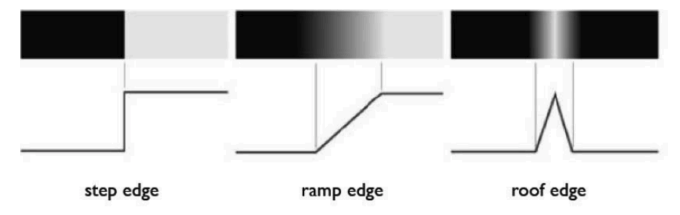
\includegraphics[width=0.75\linewidth]{images/pixel_intensity.png}
    \caption{Representation of the three types of edge that can be found in image analysis.\\Source: \cite{niebles2012edge}}
    \label{fig:pixel_intensity}
\end{figure}

\subsubsection{Gradient Computation}\label{sec:deriv_mask}

In HOG, a derivative mask (also known as a filter or kernel) is used to compute gradient information from an image \cite{dalal_2005_histograms} by performing convolution, the process of adding each element of the image to its local neighbors, weighted by the mask \cite{niebles2012edge}, as shown in equation \ref{eq:convolution}, where $I$ is the image matrix, $K$ the mask's matrix and $k$ - the "radius" of K (the distance from the center element to an edge element). 

\begin{equation}\label{eq:convolution}
    F(x,y) = \sum_{i=-k}^{k} \sum_{j=-k}^{k} I(x+i,y+j) \cdot K(i,j)
\end{equation}

%TODO: Make this discrete convolution equation actually make sense

The authors of HOG found that a simple 1D derivative mask of form $[-1,0,1]$, formally called a central discrete derivative \cite{niebles2012edge}, while being much less computationally expensive than 3x3 Sobel or 2x2 diagonal masks, also performed the best \cite{dalal_2005_histograms}.

Convolution on an image $I$ with the aforementioned 1D mask yields a new image $F_y$ defined in \ref{central_1} and convolution with the transposed, or, in other words, "flipped" over its main diagonal, 1D mask yields an image $F_x$ as defined in \ref{central_2}.

\begin{equation}\label{central_1}
    F_{y}(x_{m},y_{n}) = \frac{ \partial I(x_{m},y_{n}) }{ \partial x } \approx |\ I(x_{m}-1,y_{n})-I(x_{m}+1,y_{n})\ | 
\end{equation}
\begin{equation}\label{central_2}
    F_{x}(x_{m},y_{n}) = \frac{ \partial I(x_{m},y_{n}) }{ \partial x } \approx |\ I(x_{m},y_{n}+1)-I(x_{m},y_{n}-1)\ | 
\end{equation}

Notice however, that $x_m\pm 1$ and $y_n\pm 1$ fall outside $I[0,w-1]\times[0,h-1]$ when $x_m=w-1$ and $y_n=h-1$ respectively. This means that gradient information at image boundaries is lost when using central finite differences for convolution \cite{shidlovskiy_2020_reducing}. The information loss is evident in the \href{https://github.com/scikit-image/scikit-image/blob/main/skimage/feature/_hog.py}{\_hog\_channel\_gradient} where the convolution output at boundary pixels defaults to zero. The nullified boundary pixels may disproportionately impact SVM performance when using smaller detection windows or block sizes, as these zeroed values constitute a larger fraction of the resulting histogram. To address this limitation, this investigation proposes a novel approach that combines central, forward, and backward finite differences \cite{niebles2012edge}.

Figure \ref{fig:finite_differences} displays the kernels of each of the finite differences. Because both forward and backward differences are not anchored around the central pixel, they can be used to yield the convoluted intensity values of pixels at the top \ref{finite_top} and left \ref{finite_left}, and bottom \ref{finite_bottom} and right \ref{finite_right} edges, respectively.

\begin{figure}
    \centering
    
\includegraphics[width=0.75\linewidth]{images/finite_differences.png}
    \caption{Three types of finite differences and their corresponding derivative masks. Source: Image by me}
    \label{fig:finite_differences}
\end{figure}

\begin{equation}
    \label{finite_top}
    F_{x}[x_{m},0] =  | I(x_{m},1)-I(x_{m},0) | 
\end{equation}
\begin{equation}
    \label{finite_left}
    F_{y}[0,y_{n}] =  | I(1,y_{n})-I(0,y_{n}) 
\end{equation}
\begin{equation}
    \label{finite_bottom}
    F_{x}[x_{m},h] =  | I(x_{m},h)-I(x_{m},h-1) 
\end{equation}
\begin{equation}
    \label{finite_right}
    F_{y}[w,y_{n}] =  | I(w,y_{n})-I(w-1,y_{n}) 
\end{equation}

With the convoluted pixel values, or, in a sense, the changes in pixel intensity encoded into both $F_y$ and $F_x$ images, combining them into a single feature map $G$ of gradients, or vectors with an angle $\theta$, is as simple as applying the Pythagorean theorem \cite{shidlovskiy_2020_reducing}, as illustrated in figure \ref{fig:pythagorean}, where $ \text{magnitude} = | G(x_{m},y_{n}) | = \sqrt{ F_{y}(x_{m},y_{n})^2+F_{y}(x_{m},y_{n})^2 }$ and $\theta = \arctan \left( \frac{F_{y}(x_{m},y_{n})}{F_{x}(x_{m},y_{n})} \right) $

\begin{figure}
    \centering
    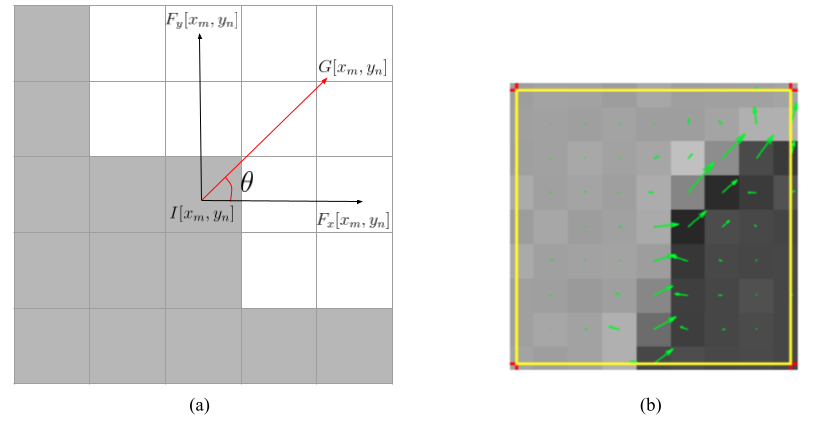
\includegraphics[width=0.75\linewidth]{images/pythagorean.png}
    \caption{(a) Calculation of gradient vector. Source: Image by me (b) Visualization of gradient vectors. Source: \cite{shidlovskiy_2020_reducing}}
    \label{fig:pythagorean}
\end{figure}

\subsubsection{Orientation Binning}

Orientation Binning hopes to achieve an encoding that is both sensitive to variations in local image content while remaining resistant to miniature changes in pose or appearance. This approach pools gradient orientation information locally, in a similar way that the SIFT feature detector does \cite{lowe_2004_distinctive}.

The process of orientation binning begins with dividing the constructed feature map of gradients into local spatial regions that the authors of the HOG algorithm called cells, as illustrated in figure \ref{fig:cells}.

\begin{figure}
    \centering
    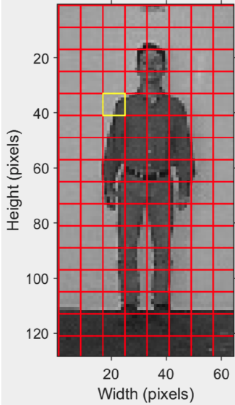
\includegraphics[width=0.3\linewidth]{images/cells.png}
    \caption{A 128x64 image divided into a grid of 8x8 pixel sized cells. Source: \cite{shidlovskiy_2020_reducing}}
    \label{fig:cells}
\end{figure}

Each pixel in a cell is characterized by its edge direction (0°-180°) and edge strength. The edge direction determines which oriented bin, $j$ (from equation \ref{eq:bin}), will receive the pixel's edge strength as its vote. These pixel-level measurements contribute to the cell's local feature vector of size $\omega$, which is essentially a histogram with $\omega$ bins evenly spaced across the 0°-180° range of possible edge orientations.

\begin{equation}
    \label{eq:bin}
    j = \left\lfloor  \left( \frac{\theta \omega}{180 \degree} \right) - \frac{1}{2}  \right\rfloor 
\end{equation}

\begin{figure}
    \centering
    
\includegraphics[width=0.75\linewidth]{images/histogram_bins.png}
    \caption{A histogram with 9 equally distributed bins. Source: Image by me}
    \label{fig:histogram_bins}
\end{figure}

While it is also viable to use 'signed' edge directions with a range of 0°-360°, it is generally unnecessary to distinguish between opposite edge directions since object classification is mainly based on detecting boundaries between regions of different intensities. Both edge directions of 90° and 270° convey the same boundary information, just with reversed intensity transitions \cite{shidlovskiy_2020_reducing}. The original HOG authors show that using signed edge directions not only fails to add useful information but actually decreases performance specifically in pedestrian detection \cite{dalal_2005_histograms}, presumably because the wide range of clothing and background color transitions obscure underlying shapes.

\subsubsection{Block Normalisation}
The magnitude of gradients can vary widely depending on local variations in illumination and foreground-background contrast. The authors of HOG thus found that local contrast normalization significantly contributes to classifier performance \cite{dalal_2005_histograms}, likely because it allows the classifier to focus on the structure of objects rather than brightness changes. It also ensures contrast invariance, balancing the influence of gradients in both high and low-contrast areas, preventing overemphasis on certain regions. Furthermore, normalization smooths the feature representation, reducing noise and making the extracted features more consistent across the image. By locally adapting to different image regions, normalization helps the classifier identify meaningful patterns and essential details.

Local contrast normalization addresses variations in illumination and contrast by first grouping the cell histograms into an unnormalized block descriptor vector, $\vec{f_{b}} = \{ b_{i} \ |\ i=1,2,\dots, c_w \cdot c_h \}$ (where $c_w$ and $c_h$ represent the number of cells in a block's width and height respectively), as illustrated in figure \ref{fig:normalisation}. While several normalization schemes exist ($\mathrm{L1}$, $\mathrm{L1-sqrt}$, $\mathrm{L2}$, and $\mathrm{L2-hys}$) \cite{dalal_2005_histograms} their impact on pedestrian detection performance is negligible. The original HOG authors found that all four schemes performed similarly, with $\mathrm{L2}$ and $\mathrm{L2-hys}$ showing only marginally better results \cite{dalal_2005_histograms}. This suggests that the choice of normalization scheme is less critical than other HOG parameters for pedestrian detection tasks.

\begin{figure}
    \centering
    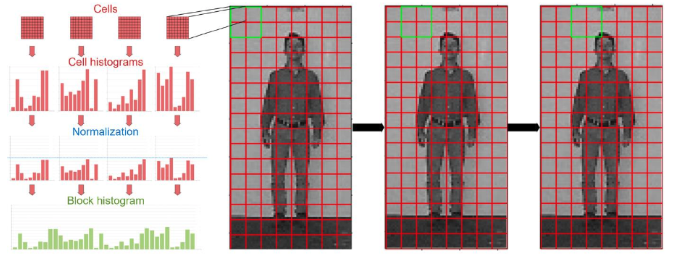
\includegraphics[width=0.75\linewidth]{images/normalisation.png}
    \caption{Construction of histogram blocks of size (2,2). Source: \cite{shidlovskiy_2020_reducing}}
    \label{fig:normalisation}
\end{figure}

One essential feature of grouping cell histograms into blocks is that the blocks themselves may overlap. Depending on the stride with which the block window moves, the horizontal and vertical overlaps will be $(1-\frac{\text{block width}}{\text{horizontal block stride}})\%$ and $(1-\frac{\text{block height}}{\text{vertical block stride}})\%$ respectively. While normalizing the same histograms in different block contexts may seem redundant, the authors of HOG found that the increased number of descriptor vectors $\vec{f_b}$ significantly improved performance \cite{dalal_2005_histograms}.

%TODO: Explain WHY it improved performance

\subsubsection{Feature Vector Dimensionality}\label{sec:feature_vector_dimensionality}

A sliding detection window is essential for object detection tasks like pedestrian classification because it allows the classifier to systematically examine all parts of the image at various positions and scales. Objects of interest, such as pedestrians, can appear at different locations, sizes, and orientations within an image, making it crucial to have a method that can effectively search across the entire image space. The sliding detection window of dimensions  $W_h$ and $W_w$ scans the image in a grid-like fashion, shifting over both horizontal and vertical axes. At each location, the window encompasses a region of interest containing a dense grid of overlapping blocks.

As the window moves across the image, the feature descriptors $\vec{f_b}$ within each block's region are computed, normalized, and combined into a larger feature vector, $\vec{L}$, as illustrated in figure \ref{fig:hog_pipeline}. The vector $\vec{L}$, representing the entire sliding window at that position, is used as input to the linear Support Vector Machine classifier to decide whether the window contains a pedestrian or not. 

\begin{figure}
    \centering
    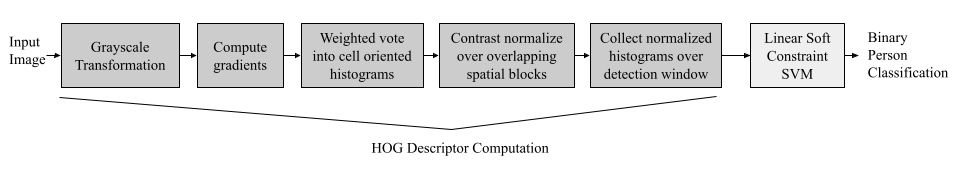
\includegraphics[width=1\linewidth]{images/HOG Pipeline.png}
    \caption{An overview of the HOG feature extraction chain. Source: Adapted by me from \cite{dalal_2005_histograms}}
    \label{fig:hog_pipeline}
\end{figure}

The dimensionality, $d$, of the vector $\vec{L}$ in essence describes the the total number of individual features, or gradients in a specific region of the image. Formally, it is said that the vector $\vec{L}$ belongs in a feature space of $d$ dimensions ($\vec{L} \in \mathcal{R}^{d}$). The higher the dimensions of this space, the more information a model has to distinguish between a pedestrian and the background or a humanoid silhouette (though this is not always the case, as explained in section \ref{sec:curse_of_dimensionality}). 

If we were to restrict the possible spatial block region's horizontal, $b_w$, and vertical, $b_h$, dimensions to even numbers, it could be easily expressed that the center coordinates, $x$ and $y$, of any block are bounded within $\left[ \frac{b_w}{2}; \frac{W_w}{c_w} - \frac{b_w}{2}\right]$ and $\left[ \frac{b_h}{2}; \frac{W_h}{c_h} - \frac{b_h}{2}\right]$ sets of cell values, respectively, as illustrated in figure \ref{fig:center_coords}

\begin{figure}
    \centering
    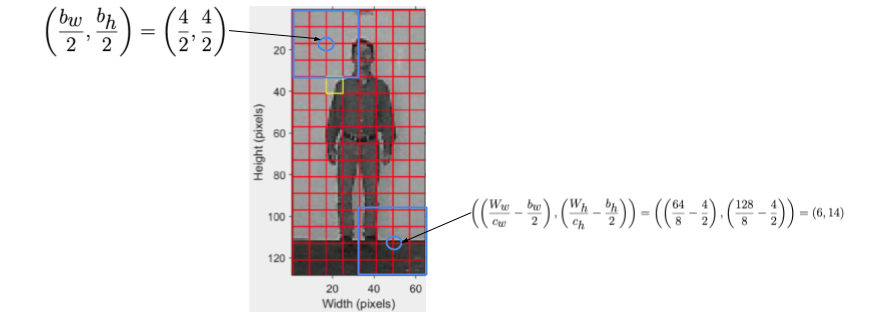
\includegraphics[width=1\linewidth]{images/Center Coordinates.png}
    \caption{A 128x64 sized image with cells that contain 8x8 pixels and blocks that contain 4x4 cells. The top left-most and bottom-right most block coordinates are each expressed using the aforementioned bounds. Source: Adapted by me from \cite{shidlovskiy_2020_reducing}}
    \label{fig:center_coords}
\end{figure}

The dimensionality $d$ of the final feature vector $\vec{L}$ depends on two factors: the size of each block descriptor $\vec{f_b}$ and the total number of blocks in the detection window. Each block descriptor's size is determined by the number of cells in the block ($c_w\cdot c_h$) multiplied by the number of orientation bins per cell ($\omega$). The number of blocks is determined by how many times a block can be shifted within the window using the horizontal and vertical stride values ($s_w$ and $s_h$). These relationships are formalized in equation \ref{vector_dimensions}.

\begin{equation}
    \label{vector_dimensions}
    \begin{split}
    d &= \left\lfloor \frac{\frac{W_w}{c_w}-2\cdot\frac{b_w}{2}+1}{s_w} \right\rfloor\left\lfloor \frac{\frac{W_h}{c_h}-2\cdot\frac{b_h}{2}+1}{s_h} \right\rfloor\cdot b_w b_h\omega \\ &= \left\lfloor  \frac{W_w- c_w(b_w-1)}{s_w c_w}  \right\rfloor \left\lfloor   \frac{W_h -c_h(b_h +-1)}{s_h c_h} \right\rfloor b_w b_h\omega
    \end{split}
\end{equation}

\subsection{Supervised Machine Learning}\label{sec:supervised_ml}

Machine Learning (ML), on a surface level, is the study of algorithms that are designed to produce outputs without an explicit instruction set generated by a person but rather with reference to the patterns or correlations found in data \cite{what_is_ml}. 

In that respect, supervised ML algorithms are a subset of ML algorithms which attempt to make predictions from data \cite{supervised_learning}. Such algorithms rely on labeled training datasets, or data sets which provide the correct outputs that an algorithm should produce for each input data point \cite {supervised_learning}. 

Supervised ML applications include classifiers, such as a pedestrian detection program, which learn from previously annotated data in the hope of predicting the "class" to which future input data will belong. \cite{derek_2020_svm}. For example, a good pedestrian classifier should be able to predict whether an image's window belongs to the class of windows that contain a pedestrian or to the class of windows that do not contain a pedestrian.

Classifier training data is formally defined as $D={ (x_{1},y_{1}),\dots,(x_{n},y_{n}) }$, where each feature vector $x$ belongs to a $d$-dimensional space ($x\in \mathcal{R}^d$) and each label $y$ belongs to a label space $\mathcal{C}$ \cite{supervised_learning}. For pedestrian detection, which is a binary classification problem, the label space contains just two values: $+1$ for pedestrians and $-1$ for non-pedestrians \cite{cornell_svm}. Since each feature vector $x$ corresponds to a HOG descriptor $\vec{L}$, any change in the HOG parameters discussed in section \ref{sec:feature_vector_dimensionality} alters the dimensionality of $\vec{L}$ and consequently requires training a new classifier model with appropriately dimensioned feature vectors.

\subsection{Support Vector Machines}

Support Vector Machines (SVM) are widely adopted supervised machine learning algorithms, particularly well-suited for high-dimensional feature spaces like those generated by HOG descriptors \cite{ng_support}. While other classification algorithms exist, such as decision trees \cite{cornell_decision_trees}, naïve bayes \cite{cornell_naive_bayes}, and deep neural networks \cite{cornell_nn}, SVMs are especially effective at finding optimal separation boundaries in high-dimensional spaces \cite{chang_lin_2011_libsvm}. Their effectiveness has been demonstrated across various domains, from medical applications like brain disorder diagnosis \cite{derek_2020_svm} and neuroimaging analysis \cite{svm_mri} to computer vision tasks, where they have become the standard classifier for HOG-based pedestrian detection \cite{dalal_2005_histograms}.

An SVM finds the optimal boundary (hyperplane) to separate data points of different classes \cite{derek_2020_svm}. This hyperplane is mathematically defined as $\mathcal{H}={ x|w^\top x + b = 0 }$, where $w$ is the weight vector and $b$ is the bias \cite{cornell_svm_notes}. While other algorithms like the Perceptron \cite{cornell_perceptron} also find separating hyperplanes, SVMs are distinguished by their goal of maximizing the margin—the distance between the hyperplane and the nearest data points (called support vectors) from each class \cite{ng_support}. Figure \ref{fig:hyperplane} illustrates this concept in two dimensions, where the hyperplane becomes a line, $w$ represents the vector perpendicular to this line, and $b$ determines the line's intercept with the y-axis.

\begin{figure}
    \centering
    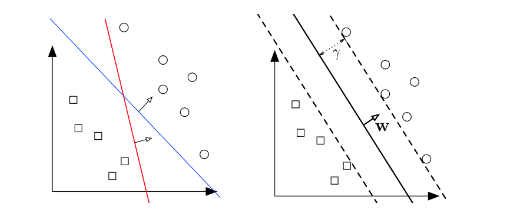
\includegraphics[width=0.75\linewidth]{images/hyperplane.png}
    \caption{A 2 dimensional space, where each data point has 2 features (one abscissa and one ordinate component) (Left:) Two different separating hyperplanes for the same data set (the multiple possibles hyperplanes of, for example, the perceptron algorithm). (Right:) The maximum margin hyperplane (the only possible hyperplane of the SVM algorithm). Source: \cite{cornell_svm_notes}}
    \label{fig:hyperplane}
\end{figure}

A hyperplane with the maximum possible margin between its support vectors is incredibly useful as it increases the likelihood of producing a generalized classifier, which can accurately separate unseen data points \cite{cornell_svm}. By expressing the distance between any point and that point's projection in the hyperplane, as illustrated in figure \ref{fig:hyperplane_geometry}, with the two variables that define the hyperplane itself (the weight and the bias), we get a definition of the margin, $\gamma$ in \ref{margin_expr} \cite{cornell_svm_notes}

\begin{equation}\label{margin_expr}
    \gamma(w,b)=\min_{x\in D} \frac{|w^\top x + b|}{||w||_{2}}
\end{equation}

\begin{figure}
    \centering
    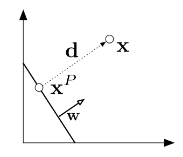
\includegraphics[width=0.35\linewidth]{images/hyperplane_geometry.png}
    \caption{The projection of a data point onto the hyperplane. Source: \cite{cornell_svm_notes}}
    \label{fig:hyperplane_geometry}
\end{figure}

With a defined margin, finding the optimal hyperplane can be formulated as a concrete optimization problem: maximize the margin $\gamma$ while ensuring all data points lie on the correct side of the hyperplane based on their class labels. The latter requirement istockphoto expressed mathematically as the inequality in equation \ref{hyper_inequality} \cite{ng_support}. For any data point $x_i$, the expression $w^\top x_i + b$ determines its position relative to the hyperplane $\mathcal{H}$: positive values indicate $x_i$ lies above $\mathcal{H}$, while negative values indicate it lies below. Therefore, when this expression is multiplied by the class label $y_i$ (which is either +1 or -1), the result should be positive for correctly classified points, providing a mathematical foundation for the optimization constraint.

\begin{equation}\label{hyper_inequality}
y_{i}(w^\top x_{i}+b)\ge 0 \quad 
\end{equation}
%TODO: Should I expand more on the concrete form of how this optimization problem looks?

\subsubsection{Soft SVM Constraints}\label{sec:soft_constraint_svm}
% Improve this paragraph
Traditionally obtaining the largest possible margin $\gamma$ would be a quadratic programming problem \cite{quadratic_programming} (as the goal of maximizing $\gamma$ is primarily anchored around minimizing $||w||_{2}$ from the equation in \ref{margin_expr} with the linear constraint in \ref{hyper_inequality}). While an SVM model's hyperplane such a "hard" constraint in \ref{hyper_inequality} could, in theory, be found found using either QCQP \cite{cornell_svm_notes} or SMO \cite{chang_lin_2011_libsvm} algorithms, in practice pedestrian datasets are incredibly noisy, as mentioned in section \ref{sec:introduction}, while also containing humanoid figures which closely approximate the features of a pedestrian \cite{inria_improved}, as visualized in figure \ref{fig:manequin_features}. Because of noise and obfuscation in real world pedestrian data, an SVM with a hard linear constraint would fail to compute the optimal hyperplane as there would be a significant number of outliers or data points which share features common to both classes, as illustrated in figure \ref{fig:outliers}. Instead, in the hope of finding a hyperplane that achieves the best realistically possible classification accuracy, an SVM with a soft constraint, which does allow for some degree of error while maximizing $\gamma$, ought to be used \cite{dalal_2005_histograms} \cite{cornell_svm_continued}.

\begin{figure}
    \centering
    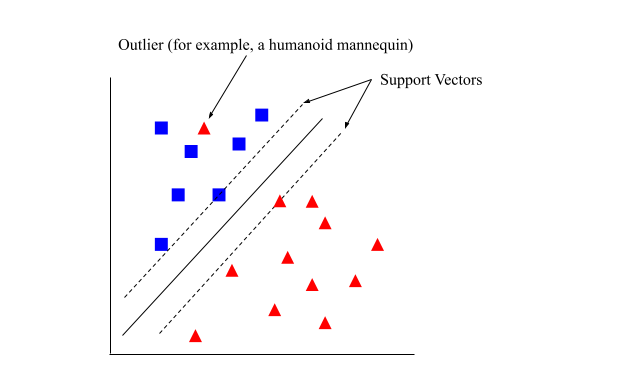
\includegraphics[width=0.75\linewidth]{images/outliers.png}
    \caption{A Data set with two classes and an outlier. Source: Image by me}
    \label{fig:outliers}
\end{figure}

\begin{figure}
    \centering
    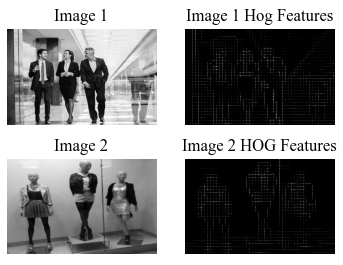
\includegraphics[width=0.75\linewidth]{images/features.png}
    \caption{(Image 1: ) An Image containing three people/pedestrians in a building. Source: \href{https://www.istockphoto.com/photo/business-people-taking-a-break-gm639259132-115111535}{istockphoto.com} (Image 2:) An Image containing three mannequins in a store window. Source: \href{https://theshopcompany.com/blog/Mannequins_and_Dressforms_Who_Uses_What}{theshopcompany.com} (Image 1 and 2 Hog Features): Computed HOG Features of Image 1 and Image 2. Source: Image by me}
    \label{fig:manequin_features}
\end{figure}

% TODO: Will I even be able to explain how to maximise the margin?

\subsection{The Curse of Dimensionality}\label{sec:curse_of_dimensionality}

While it would be reasonable to intuitively to assume that the more information, or vector dimensions, a machine is provided during training, the more accurate it would be at classification tasks, the classic "curse of dimensionality" problem shows that this is not necessarily the case \cite{jain_1982_39} \cite{friedman_1997_on}, as overfitting, the process of fitting to noise rather than underlying patterns, \cite{overfitting} occurs when the amount of "specific information" (the dimensions of each data point's vector $\vec{L}$) is significantly greater than "global information" (the amount of data points in a data set) \cite{overfitting} \cite{liu_2016_overfitting}, as shown in figure \ref{fig:curse_dim}. 

\begin{figure}
    \centering
    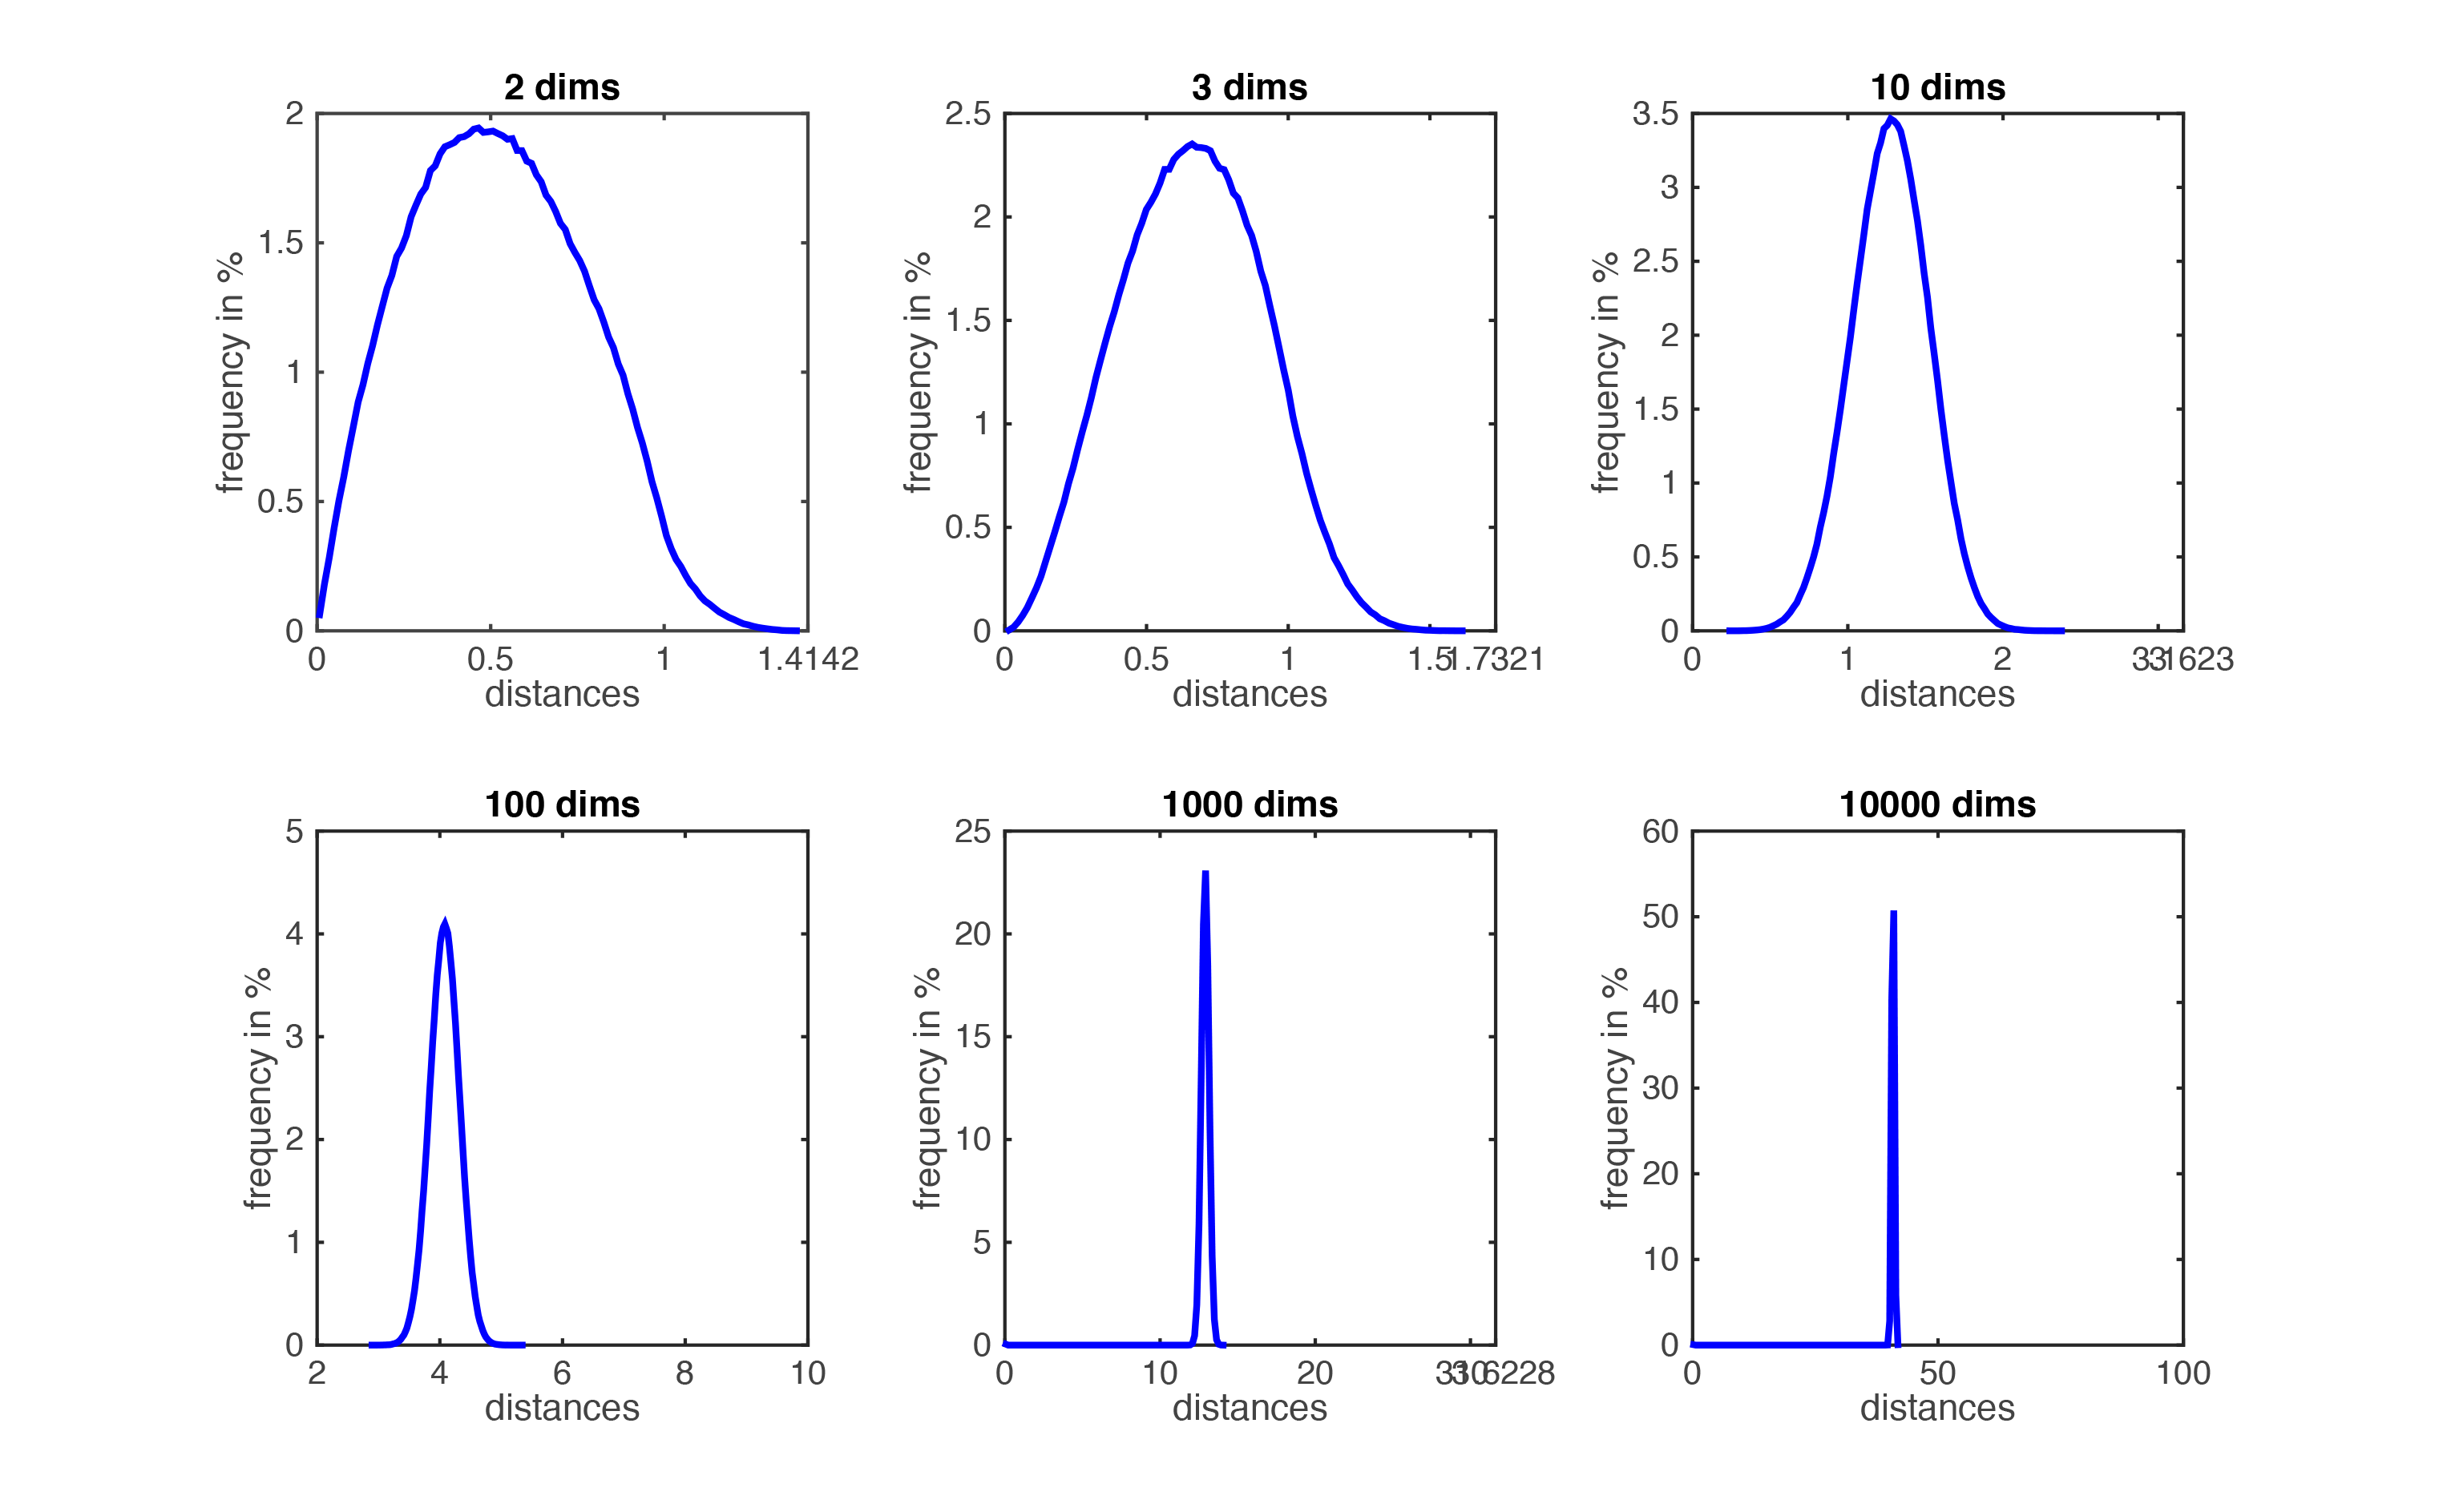
\includegraphics[width=\linewidth]{images/cursefigure.png}
    \caption{Multiple graphs which demonstrate the "curse of dimensionality". The histogram plots show the distributions of all pairwise distances between randomly distributed points within $d$-dimensional unit squares. As the number of dimensions $d$ grows, all distances concentrate within a very small range. Source: \cite{cornell_curse_notes}
}
    \label{fig:curse_dim}
\end{figure}



\section{Methodology}

\subsection{Dependant Variables}\label{sec:dependent_variables}

As mentioned in section \ref{sec:supervised_ml}, whenever any of the components of a feature vector's dimensionality, as defined in \ref{vector_dimensions}, changes, a new model has to be trained. The values for which various sets of HOG parameters will be tested in this investigation are listed in table \ref{table:dependent_variables}. Notice that the use of a "holistic" derivative mask, as introduced in section \ref{sec:deriv_mask} and implemented in appendix \ref{appendix:holistic_der_mask}, is also listed as a dependent variable. While the derivative mask which is used does not change a vector's dimensions it does change the vector's shape and, given the novel approach, it is nonetheless important to test how an SVM reacts to a differently shaped HOG descriptor. 

\begin{table}
\renewcommand{\arraystretch}{1.0}
\begin{tabular}{@{} l @{\hspace{1cm}} l @{}}    
    \toprule
    \emph{Parameter} & \emph{Values}  \\\midrule
    Window Dimension Pairs ($W_h$,$W_w$)             & (100, 50), (128, 96), (128, 64), (112, 48)  \\ 
    Cell Histogram Bin Counts ($\omega$)              & 9, 13, 18  \\ 
    Cell Dimension Pairs ($c_w$,$c_h$)           & (4,4), (6,6), (8,8), (10,10)  \\ 
    Block Dimension Pairs ($b_w$,$b_h$)           & (1,1), (2,2), (3,3), (4,4)  \\ 
    Block Stride Dimension Pairs ($s_w$,$s_h$)              & (1,1), (2,2), (3,3)  \\ 
    Holistic Derivative Mask (appendix \ref{appendix:holistic_der_mask}) & True, False  \\\bottomrule
\end{tabular}
\caption{Dependent variables for the experiment}
\label{table:dependent_variables}
\end{table}

The only restriction on the values in table \ref{table:dependent_variables} that can be combined to a set of HOG parameters is $b_w\ge s_w$ and $b_h\ge s_h$, since the use of blocks with stride values greater than block dimensions would result in certain cells being simply ignored for in the resultant feature vector $\vec{L}$. With the restriction, the number of different sets of values is given by $N$ in equation \ref{eq:number_sets}.

\begin{equation}\label{eq:number_sets}
\begin{split}
N &= |\{(W_h, W_w)\}| \times |\{\omega\}| \times |\{(c_w, c_h)\}| \times 2 \times \sum_{\substack{b_w \geq s_w \\ b_h \geq s_h}} |\{(b_w, b_h)\}| \times |\{(s_w, s_h)\}|  \\
&= 4 \times 3 \times 4 \times 2 \times 9  =864
\end{split}
\end{equation}

\subsection{Data Sets}

\subsubsection{Labeled Pedestrian Data Set Sources}

Many past studies which have evaluated the HOG approach to feature detection have heavily \cite{piotrdollr_2012_crosstalk} or, in some cases \cite{zhou_2021_research}, solely relied on the INRIA pedestrian dataset \footnote{URL for the INRIA dataset (the original web page which provided the data set is, as of 2024 October 23rd, not accessible, thus a copy from \href{kaggle.com}{kaggle} is used): \url{https://www.kaggle.com/datasets/jcoral02/inriaperson}.}, as it has been the most popular data set for pedestrian detection algorithm evaluation \cite{dollar_2012_pedestrian} since HOG features were first introduced \cite{dalal_2005_histograms}. Nevertheless, there are flaws with the data set, mainly in the limited annotation: many people which appear in test images are not labelled, estimates of each person’s visibility are lacking, and there are no class labels for the regions of the images that contain ambiguous objects \cite{inria_improved}. Matteo Taiana et al introduced an improved iteration of INRIA with labelling that addresses the aforementioned issues and, as such, their improved INRIA data set \footnote{URL for the improved inria labels: \url{http://users.isr.ist.utl.pt/~mtaiana/data.html}.} will be used in this essay's experiment.

Aside from the shortcomings of labelling in INRIA, the dataset is biased toward large, mostly unoccluded pedestrians \cite{dollar_2009_pedestrian}. The majority of people found in the dataset’s images are at a scale such that their limbs are 6 to 8 pixels wide \cite{dalal_2005_histograms}, which can undoubtedly introduce confirmation bias when attempting to evaluate the most performant cell size. As the goal of this investigation is to find a HOG descriptor that performs the best in real world environments, a greater variety of scales and occlusions will be introduced with the use of the more challenging and larger Caltech Pedestrian Dataset \cite{dollar_2009_pedestrian}, which contains richly annotated, low-resolution images of frequently occluded people. Images in real world applications may also include objects, like mannequins or statues, which closely resemble humanoid features, as previously shown in figure \ref{fig:manequin_features}. Neither INRIA nor the Caltech datasets contain such objects and thus a different dataset which addresses the range of false positive in pedestrian detection by providing labelled images with "person-like" objects \cite{karthika_2020_addressing} is also used in the investigation.

\subsubsection{Caltech Data Set Transformation}\label{sec:caltech_trasnform}

The PASCAL VOC challenges \cite{everingham_2009_pascal} introduced numerous standards in image classification, including the Pascal VOC labelling format, which has become the preferred scheme in many object classification applications, including pedestrian detection \cite{dollar_2012_pedestrian}. Both INRIA and the PnPLO (person-like) datasets abide this format, however the Caltech data set, since it's comprised of annotated videos rather than images, uses video bounding box labels \cite{mathworks_vbbLabeler}, which are especially useful for applications which involve tracking. This investigation, however, is only concerned with the detection of a pedestrian in an image, and because of that, the video (seq) files and video bounding box annotation (vbb) files are converted to images and Pascal VOC format xml files (appendix \ref{appendix:caltech_transform}). 

Besides differences in annotation, the Caltech data set videos contain $\sim 250,000$ frames \cite{dollar_2009_pedestrian}, which vastly outnumbers the $1085$ images in INRIA \cite{dalal_2005_histograms} and $1339$ images in PnPLO \cite{karthika_2020_addressing}. Given both the great quantity of data in Caltech frames and the large amount of models (864 from equation \ref{eq:number_sets}) that would need to be trained on that data, it becomes apparent that to obtain a training time that is feasible for the computational resources that can be utilized in this investigation, the amount of frames needs to be reduced. 

The total running time of the Caltech videos is $\sim 10\mathrm{h}$ \cite{dollar_2009_pedestrian}, this gives a frame per second rate of $\sim 7 \text{ frames}/\mathrm{s}$. Since a person is present in a video for $\sim 5 \mathrm{s}$ \cite{dollar_2009_pedestrian}, we can approximate that each identifiable individual will, on average, be present in $34 \text{ frames}$ and thus retaining only the $30$th frame of each video, as done in appendix \ref{appendix:caltech_30_frame}, should not incur a greatly significant cost on the amount of unique training data. By also removing frames that include the label "person?" (line 193 of appendix \ref{appendix:caltech_transform}), which denotes ambiguous pedestrian figures, the sum of Caltech frames is significantly reduced to $8538$.

\subsubsection{Window Size Samples}

Dalal and Triggs proposed evaluating a detector by classifying cropped windows centered on pedestrians and comparing them to windows sampled at a fixed density from non-pedestrian images \cite{dalal_2005_histograms}, thereby eliminating the need to merge nearby detections, using methods like non maximal suppression (NMS), or other post-processing steps. Figure \ref{fig:dataset_high} shows a high level overview of per-window data set preparation.

\begin{figure}
    \centering
    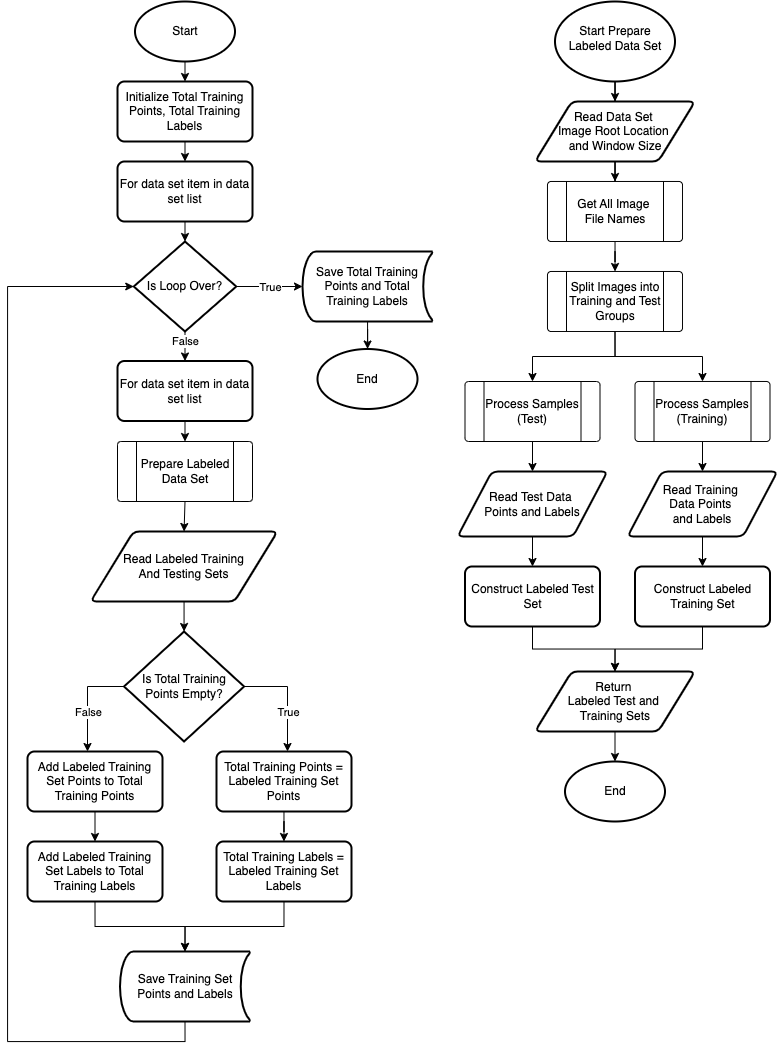
\includegraphics[width=0.75\linewidth]{images/ee_dataset_high.drawio.png}
    \caption{A high level overview flowchart of the process of initializing and saving the total training points and labels alongside each data set's testing points and labels}
    \label{fig:dataset_high}
\end{figure}

2 major concerns, however, have been raised with per-window evaluation: 
\begin{enumerate}
    \item NMS may reduce the number of false positives at varying rates for different detection methods \cite{dollar_2009_pedestrian}
    \item The per-window scheme usually relies on the use of cropped positives (windows where a pedestrian is neatly bounded) and uncropped negatives (windows that are not specifically cropped to contain random objects or background scenery). Classifiers may exploit this window boundary effect as discriminative features leading to good per-window performance but poor performance in real life applications \cite{dollar_2009_pedestrian}
\end{enumerate} 

While concern nr. 1 should not impede this investigation's goal of finding the optimal HOG parameters, as each instance of HOG interacts in a similar fashion with NMS \cite{dalal_2005_histograms}, concern nr. 2 is addressed to some degree in line 162 of appendix \ref{appendix:dataset} by applying random value paddings to the bounding boxes that comprise positive samples. This process is further explained in figure \ref{fig:dataset_low}.

\begin{figure}
    \centering
    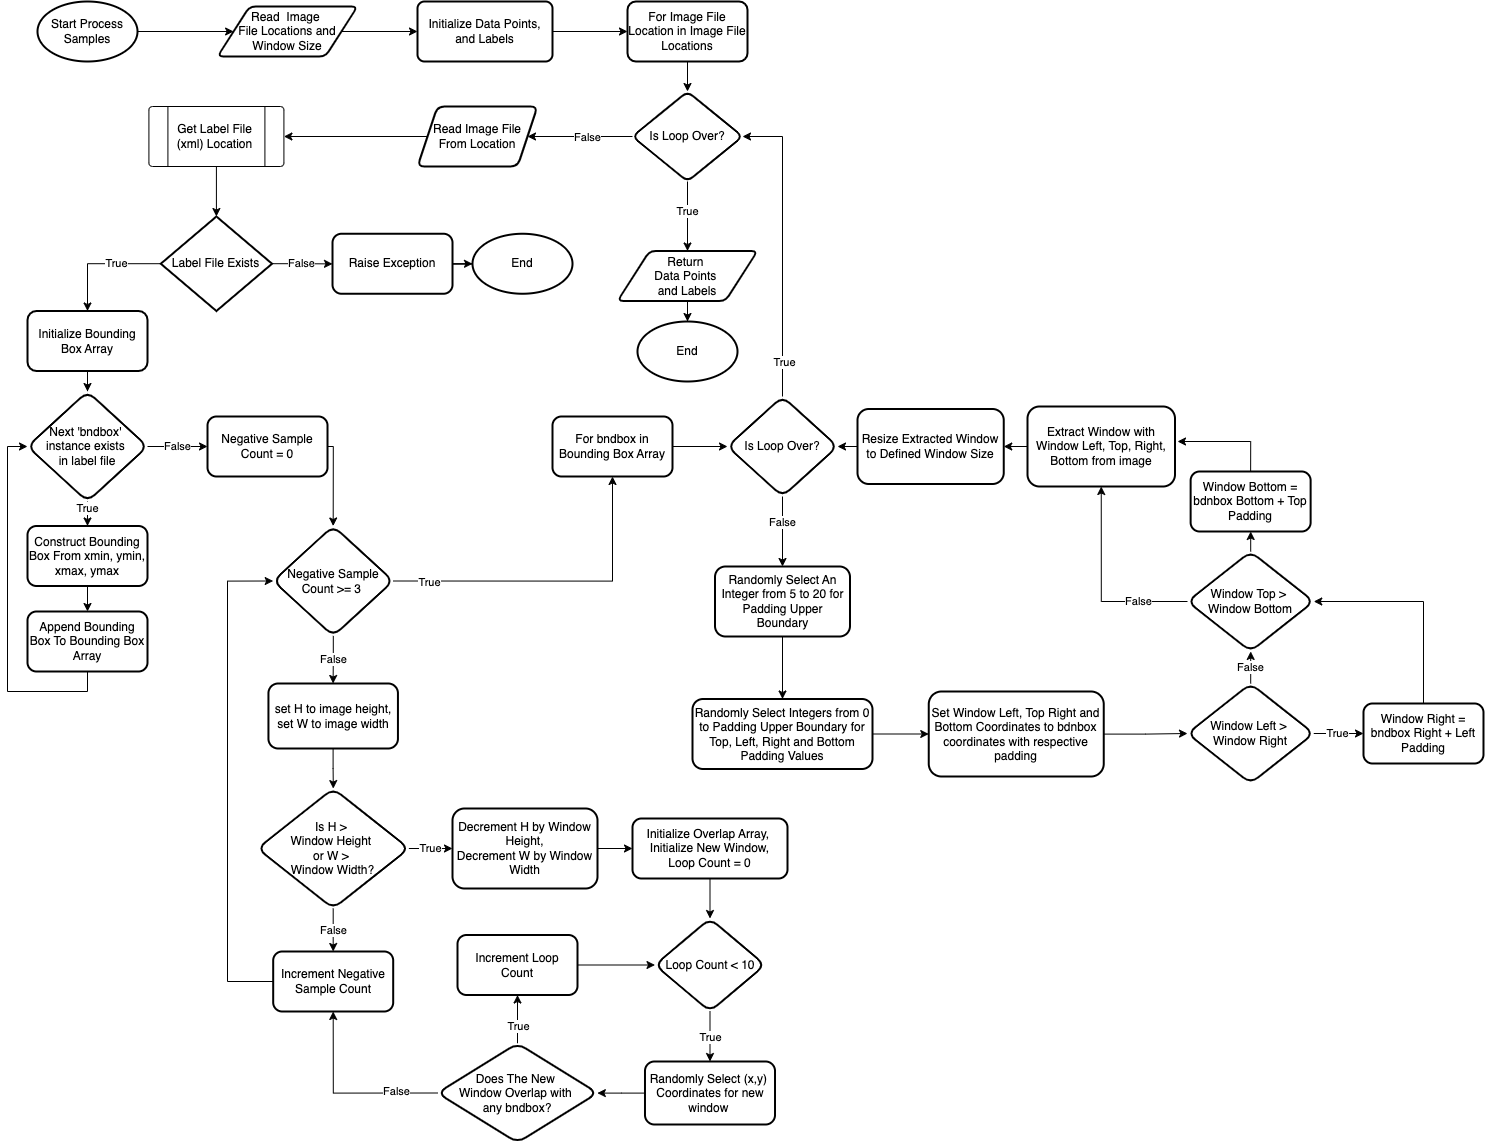
\includegraphics[width=\linewidth]{images/ee_dataset_low.drawio (1).png}
    \caption{A flowchart of the process of extracting the positive data samples (with some degree of random padding to avoid cropped positive bias) and the process of constructing negative samples }
    \label{fig:dataset_low}
\end{figure}

By using an 80/20\% training-testing data split, the number of images from section \ref{sec:caltech_trasnform} yields the numbers of different window size samples, as specified in table \ref{table:window_size_samples}

\begin{table}[H]    
    \begin{minipage}{.5\linewidth}
    \renewcommand{\arraystretch}{1.0}
    \centering
        \begin{tabular}{@{} l @{\hspace{0.5cm}} l @{\hspace{0.5cm}} l @{}}    
            \toprule
            \emph{Window Set} & \emph{Positive} & \emph{Negative}  \\\midrule
            INRIA Testing & 361 & 543  \\ 
            Caltech Testing & 2195 & 2558  \\ 
            PnPLO Testing & 596 & 578  \\
            Total Training & 12794 & 14760 \\\bottomrule
        \end{tabular}
        \subcaption{Window Size (100, 50)}
    \end{minipage}%
    \begin{minipage}{.5\linewidth}
    \renewcommand{\arraystretch}{1.0}
    \centering
        \begin{tabular}{@{} l @{\hspace{0.5cm}} l @{\hspace{0.5cm}} l @{}}    
            \toprule
            \emph{Window Set} & \emph{Positive} & \emph{Negative}  \\\midrule
            INRIA Testing & 361 & 533  \\ 
            Caltech Testing & 2195 & 2548  \\ 
            PnPLO Testing & 596 & 475  \\
            Total Training & 12794 & 14185 \\\bottomrule
        \end{tabular}
        \subcaption{Window Size (128, 96)}
    \end{minipage}%

    \vspace{1cm} % Space between rows of mini pages

    \begin{minipage}{.5\linewidth}
    \renewcommand{\arraystretch}{1.0}
    \centering
        \begin{tabular}{@{} l @{\hspace{0.5cm}} l @{\hspace{0.5cm}} l @{}}    
            \toprule
            \emph{Window Set} & \emph{Positive} & \emph{Negative}  \\\midrule
            INRIA Testing & 361 & 540  \\ 
            Caltech Testing & 2195 & 2554  \\ 
            PnPLO Testing & 596 & 535  \\
            Total Training & 12794 & 14511 \\\bottomrule
        \end{tabular}
        \subcaption{Window Size (128, 64)}
    \end{minipage}%
    \begin{minipage}{.5\linewidth}
    \renewcommand{\arraystretch}{1.0}
    \centering
        \begin{tabular}{@{} l @{\hspace{0.5cm}} l @{\hspace{0.5cm}} l @{}}    
            \toprule
            \emph{Window Set} & \emph{Positive} & \emph{Negative}  \\\midrule
            INRIA Testing & 361 & 543  \\ 
            Caltech Testing & 2195 & 2558  \\ 
            PnPLO Testing & 596 & 574  \\
            Total Training & 12794 & 14731 \\\bottomrule
        \end{tabular}
        \subcaption{Window Size (112, 48)}
    \end{minipage}%
\caption{Positive And Negative Window Samples For Each Data Set at Each Window Size.}
\label{table:window_size_samples}
\end{table}

\subsection{Evaluation Metrics}

\subsubsection{The Basic Confusion Matrix Rates}
In essence, all evaluation metrics of binary classification rely on the values of the confusion matrix, a $2 \times 2$ contingency table where the positive elements correctly classified as positives are called true positives (TP), the negative elements wrongly classified as positive are called false positives (FP), the negative elements correctly classified as negatives are called true negatives (TN), and the positive elements wrongly classified as negatives are called false negatives (FN), as shown in figure \ref{fig:conf_matrix}. \cite{chicco_eval_2023}. 

\begin{figure}
    \centering
    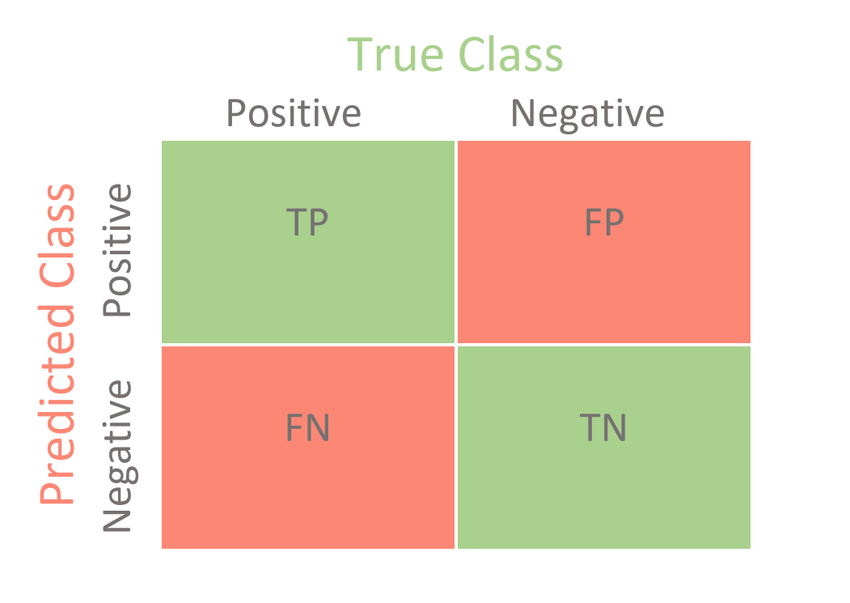
\includegraphics[width=0.5\linewidth]{images/conf_matrix.png}
    \caption{An example of a confusion matrix for binary classification. Source: \cite{conf_matrix}}
    \label{fig:conf_matrix}
\end{figure}

The four basic rates for confusion matrices are as follows \cite{chicco_eval_2023}:
\begin{enumerate}
    \item Sensitivity, or True Positive Rate, $\mathrm{TPR}=\frac{\mathrm{TP}}{\mathrm{TP}+\mathrm{FN}}$

    \item Specificity, or True Negative Rate, $\mathrm{TNR}=\frac{\mathrm{TN}}{\mathrm{TN}+\mathrm{FP}}$
    
    \item Precision, or Positive Predictive Value, $\mathrm{PPV}=\frac{\mathrm{TP}}{\mathrm{TP}+\mathrm{FP}}$
    
    \item Negative Predictive Value, $\mathrm{PPV}=\frac{\mathrm{TN}}{\mathrm{TN}+\mathrm{FN}}$
\end{enumerate} 

\subsubsection{Confidence Threshold Curves}

Many scoring classifiers produce a real-valued prediction score for each data point and, by assigning a particular threshold value $\tau$ a confusion matrix is generated for such a classifier \cite{chicco_jurman_2020_mcc_f1}. To summarize the confusion matrix, it is common to to plot one of the aforementioned four basic rates on a cartesian plane at varying $\tau$ values, like plotting a ROC curve (where TPR is plotted against the false positive rate $\mathrm{FPR}=\frac{\mathrm{TN}}{\mathrm{TN}+\mathrm{FP}}$) or the DET curve (FN rate against FP rate) which is more widespread in pedestrian detection literature \cite{dalal_2005_histograms} \cite{dollar_2012_pedestrian}. 

However, unlike methods such as logistic regression \cite{cornell_log_regression_notes}, which classify a window into one of two classes by estimating the probability that the window belongs to each class, an SVM is not a "probabilistic" model as it simply plots the window's feature vector in a space separated by a hyperplane, and thus there's no probabilistic/scoring confidence $\tau$ involved. While it's possible to compute the probabilities of an SVMs prediction using cross-validation in Platt Scaling \cite{platt1999probabilistic}, the operation is known to be very expensive for large datasets \cite{scikit-learn_svm} alongside being inconsistent with the actual predictions of the SVM \cite{scikit-learn_svm}. Nevertheless, plots with varying $\tau$ values can be extremely informative \cite{martin1997det} \cite{scikit-learn_svm} and thus instead of "probabilities", the distances from each data point to the hyperplane are used as a sort of "confidence" value.

\subsubsection{Matthew's Correlation Coefficient}

While ROC curves (or their DET counterparts) alongside the scalar value of area under the ROC curve (AUC-ROC) are very widespread, they are also fundamentally flawed in that they ignore precision since, fundamentally, AUC-ROC only identifies how well a classifier separates the positive class from the negative class, not how accurate the separation is (a metric which is ever more important in a field like pedestrian detection). Historically, precision recall curves were used to account for the drawbacks of ROC \cite{chicco_jurman_2020_mcc_f1}. Quite recently, however, the Matthew's Correlation Coefficient has been proposed as a standard metric for validating biomedical image analysis by an international group of researchers in the field \cite{Maier_Hein_2024_mcc_proposal}, primarily because it is the only rate that maximizes all four of the aforementioned basic rates \cite{Maier_Hein_2024_mcc_proposal} \cite{chicco_eval_2023} \cite{chicco_jurman_2020_mcc_f1} and is claimed to be the most informative single score to establish the quality of a binary classifier prediction \cite{chicco_eval_2023}. Because of its discriminatory power, the MCC and a corresponding MCC-F1 curve (explained in more detail in figure \ref{fig:mcc_f1_example}) will be the primary evaluation metrics used in this investigation. 

\begin{figure}
    \centering
    \includesvg[width=0.8\linewidth]{images/mcc_f1_example.svg}
    \caption{An example of an MCC-F1 curve. Unit-normalized Matthews correlation coefficient (MCC) plotted against the F1 score (the harmonic mean between precision and recall). The random line indicates that a random classifier can achieve a unit-normalized MCC of 0.5. The point of perfect performance is (1,1), representing an ideal classifier that correctly classifies every instance. Conversely, the point of worst performance is (0,0), attained by a classifier that misclassifies all instances. The best threshold point is the location on the curve that is nearest to (1,1). 5 various threshold $\tau$ values are scattered along the curve. Source: Image by Me, generated with code in appendix \ref{appendix:mcc_f1_curves}}
    \label{fig:mcc_f1_example}
\end{figure}


\begin{figure}
    $$\mathrm{MCC} = \frac{\mathrm{TP}\cdot\mathrm{TN}-\mathrm{FP}\cdot\mathrm{FN}}{\sqrt{(\mathrm{TP}+\mathrm{FP})\cdot(\mathrm{TP}+\mathrm{FN})\cdot(\mathrm{TN}+\mathrm{FP})\cdot(\mathrm{TN})+\mathrm{FN}}}$$ 
    \caption{The equation for Matthew's Correlation Coefficient. The values of MCC are bounded within the range $[-1;1]$, where 1 represents a perfect prediction, 0 represents random prediction and -1 total disagreement between prediction and observation. Refer to \cite{chicco_jurman_2020_mcc_f1} regarding the necessary normalization to make the MCC values bounded within $[0;1]$ so that they can be plotted against F1 scores (which themselves are bounded in $[0;1]$)}
\end{figure}

Nevertheless, since much of the literature on pedestrian detection and classification has historically relied on the aforementioned metrics of AUC-ROC, Average Precision and simple Accuracy \cite{dalal_2005_histograms} \cite{dollar_2012_pedestrian}, they are retained to facilitate direct and simple comparison with previous studies.

\subsubsection{McNemar's Test for Pairwise Classifier Comparison}

There are many ways to perform pairwise classifier comparison, such as conducting $5 \times 2$ Cross Validation (CV), which has historically been the preferred scheme in object classification \cite{dietterich_1998_mcnemar}. However, $5 \times 2$ CV, as the name implies, needs to be executed 10 times, while a test like McNemar's requires only a single execution. McNemar's test is also a more attractive choice as it performs increasingly better with larger datasets \cite{raschka_2018_mcnemar}. Additionally, it utilizes a version of the familiar confusion matrix, illustrated in Figure \ref{fig:confusion_mcnemar}.

\begin{figure}
    \centering
    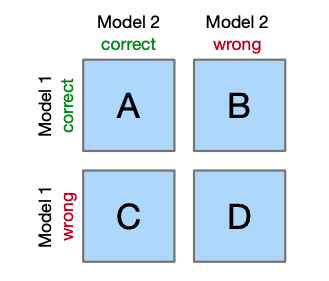
\includegraphics[width=0.5\linewidth]{images/mcnemar_matrix.png}
    \caption{Confusion matrix layout in the context of McNemar's test. Source: \cite{raschka_2018_mcnemar} Code for the construction of such a matrix can be found in appendix \ref{appendix:mcnemar}}
    \label{fig:confusion_mcnemar}
\end{figure}

McNemar's test checks if two classifiers have significantly different performance by comparing their disagreement on predictions in the confusion matrix. It calculates a p-value, the probability that the observed difference in performance is due to chance, based on a chi-square statistic \cite{dietterich_1998_mcnemar}. Typically, all p-values $\ge 0.05$ indicate that the difference between performance is not significant \cite{raschka_2018_mcnemar} \cite{dietterich_1998_mcnemar}. 

% TODO: Should I talk more about p-value and the null hypothesis?

\subsection{Model Preparation}

As mentioned in sections \ref{§sec:supervised_ml} and \ref{sec:dependent_variables}, a data set has to be uniquely prepared for each of the different 864 SVM models. This is done in two steps: by first preprocessing each window sample and then computing the HOG features (data points) on which a model will be trained and tested.

\subsubsection{Preprocessing: Grayscale Image Transformation}

The only preprocessing step used in the original HOG paper was gamma/color normalization \cite{dalal_2005_histograms}. While the paper did show that there are modest variations in classifier accuracy depending on whether an RGB, LAB or grayscale color space is used, it was also shown that the difference in illuminance became even more negligible once block normalization was applied \cite{dalal_2005_histograms}. Thus, for the sake computational simplicity, 3-channeled data points are first transformed to grayscale color spaces.

Given the rather ambiguous nature of assessing which specific method of RGB to grayscale conversion produces universally desirable outputs for all involved input images \cite{madk_2008_perceptual}, a simple and widely adopted color mapping defined in equation \ref{eq:colour_map} is used in appendix \ref{appendix:grayscale}

\begin{equation}\label{eq:colour_map}
    Y \leftarrow 0.2125 \cdot R + 0.7154 \cdot G + 0.0721 \cdot B
\end{equation}

\subsubsection{Computing HOG Features}

While an in depth explanation of how HOG features are computed was presented in section \ref{sec:hog}, there are a few notes to be made regarding the implementation of HOG in this investigation.

Since neither the \href{https://scikit-image.org/}{scikit-image} nor \href{https://opencv.org/}{OpenCV} libraries provide an implementation of HOG which would allow changing the block stride values, a custom implementation of the algorithm can be found in appendix \ref{appendix:hog}, with figure \ref{fig:hog_flowchart} providing a technical overview. The two parts of the hog pipeline (from figure \ref{fig:hog_pipeline}) that have still been reused from \href{https://scikit-image.org/}{scikit-image} are the distribution of votes to histogram bins and block normalization, as shown in figure \ref{fig:hog_flowchart}. This is primarily because both parts are highly optimized using \href{https://cython.org/}{Cython}. Even while the votes are not distributed using equation \ref{eq:bin}, giving a time complexity of $\mathcal{O}(\omega \cdot c_h \cdot c_w)$ instead of $\mathcal{O}(c_h \cdot c_w)$, the speed of the library's Cython implementation outperforms anything that would be possible using regular python.

\begin{figure}
    \centering
    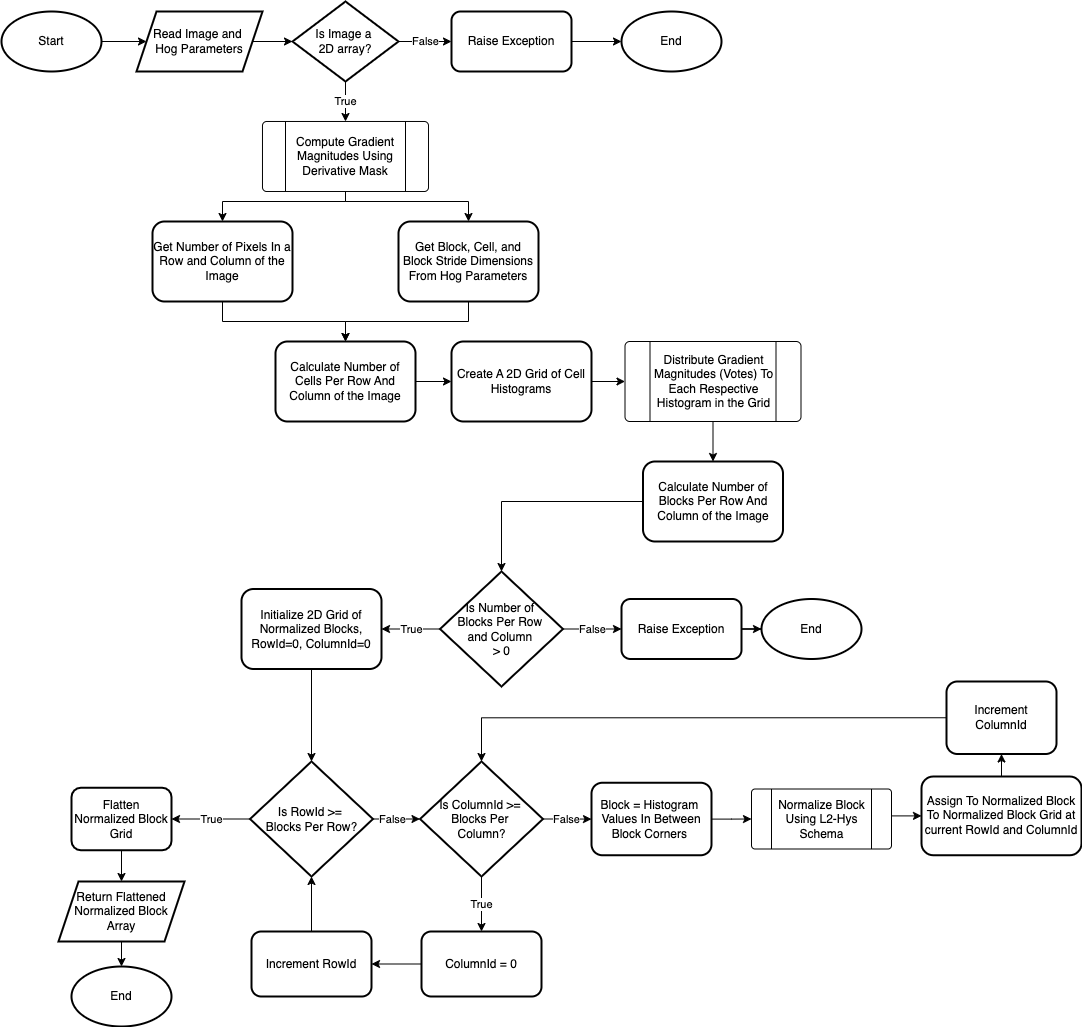
\includegraphics[width=0.85\linewidth]{images/ee_hog.drawio.png}
    \caption{A flowchart of the process of computing HOG features with custom block stride values}
    \label{fig:hog_flowchart}
\end{figure}

\subsubsection{Choosing an SVM}\label{sec:svm_choice}

The primary factor driving the choice of SVM implementation is time of computation. Given the relatively large number of models that have to be trained on $\sim$ 27,000 samples, an implementation which is able to maximize the hyperplane's margin in the least amount of time while still maintaining relatively decent classification performance is a necessity. 

The standard SVM implementation is LibSVM \cite{chang_lin_2011_libsvm} \cite{scikit-learn_svm}, however, it's training times scale quadratically with the number of samples \cite{scikit-learn_svm} (in practice it takes $\sim$ 1,600,000 \% more time to train an SVM with SMO as opposed to SGD \cite{sgd_leon}). The maintainers \href{https://scikit-learn.org/}{scikit-learn} recommend using either LibLinear or their own implementation of a linear SVM with stochastic gradient descent (SGD). SGD only uses a subset of samples when determining the cost function's, which, in this case, has inputs of §$||w||_{2}$ and $b$ from section \ref{sec:soft_constraint_svm}, gradient and the subsequent direction towards the global minima \cite{uc_berkeley_sgd}. This is in contrast to regular gradient descent (GD) which uses all samples for gradient calculation. As such, while training a model with SGD would be faster, we should also expect the SGD model to have worse performance guarantees than GD \cite{uc_berkeley_sgd}.

In practice however, both LibLinear \footnote{LibLinear SVM docs: \url{https://scikit-learn.org/1.5/modules/generated/sklearn.svm.LinearSVC.html}} and an SVM with GDC \footnote{SVM with SGD docs: \url{https://scikit-learn.org/1.5/modules/generated/sklearn.linear_model.SGDClassifier.html}} exhibit essentially identical pedestrian classification performance, as evidenced by a McNemar's test p-value of $\sim$ 0.121, further comparisons are made in table \ref{tab:liblinear_vs_sgd_table} and figure \ref{fig:liblinear_vs_sgd_curve}.

\begin{table}
    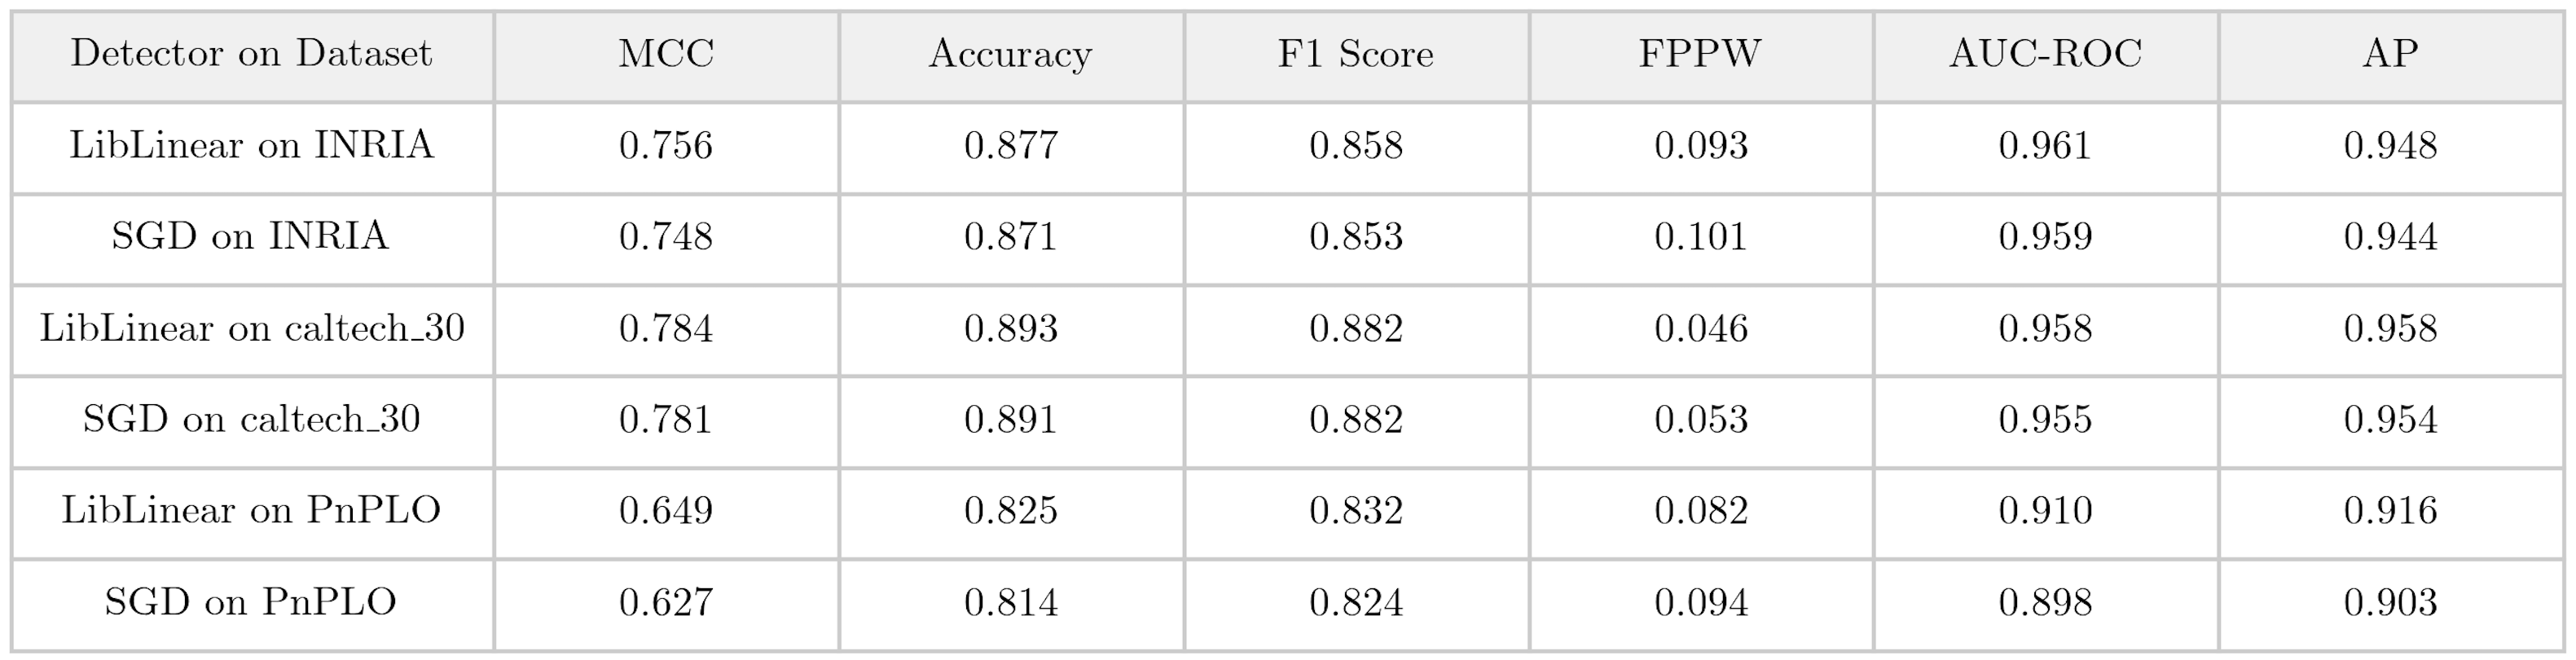
\includegraphics[width=\linewidth]{images/liblinear_vs_sgd_table.png}
    \caption{The evaluation metrics of a LinearSVC and SGDClassifier SVM implementations, trained on the standard HOG feature parameters \cite{dalal_2005_histograms}: $128\times64$ windows with $8\times8$ pixels per cell, $2\times2$ cells per block, $1\times1$ block strides. Source: Image by Me, generated with code in appendix \ref{appendix:evaluate_metrics}}
    \label{tab:liblinear_vs_sgd_table}. 
\end{table}


\begin{figure}
    \centering
    \includesvg[width=0.75\linewidth]{images/liblinear_vs_sgd_curve.svg}
    \caption{An MCC-F1 curve of both LinearSVC and SGDClassifier trained on the standard HOG feature parameters \cite{dalal_2005_histograms}. Notice that the best performing $\tau$ value for SGDClassifier is negative, as $\tau$ identifies the distance which allows a point to be classified as a positive. This relates to Soft Constraint SVMs mentioned in section \ref{sec:soft_constraint_svm}.}
    \label{fig:liblinear_vs_sgd_curve}
\end{figure}

\subsubsection{Training an SVM}

The code in appendix \ref{appendix:training_svm} implements SVM training using SGDClassifier optimized through cross 5-fold validation (with GridSearchCV) \cite{cornell_hyperoptimization}, which systematically explores different regularization strength values (alpha). The search grid consists of 4 "soft" regularization parameters, as discussed in section \ref{sec:soft_constraint_svm}. This means that each SGDClassifier will be fitted a total of 20 times, with the best performing model (in terms of MCC) being saved for each set of HOG parameters. While the initial learning rate (eta$\theta$) is also a parameter that should be optimized, this investigation avoids the additional training overhead by using Leon Bottou's "optimal heuristic" for deriving the learning rate from alpha \cite{sgd_leon}.

The majority of the training was performed on a linux-based system with an Intel Xeon CPU @ 2.20GHz (2 cores), 12.7GB of RAM, as provided by \href{https://colab.research.google.com/}{Google Colab}. Especially high dimensional HOG features (from figure \ref{fig:dimension_distribution}) tend to exceed the memory capacity of google colab's free tier, which is why the training for higher dimensional models was done on a local machine with an Intel Core i7 @ 2.6GHz (6 cores) and 32GB of RAM.

\begin{figure}
    \includesvg[
        width=\linewidth,
    ]{dimension_distribution.svg}
    \caption{Kernel Density Estimation (KDE) of Dimension Values generated from various Histogram of Oriented Gradients (HOG) parameters. The blue line represents the KDE trend of the dimensions, while the red dots indicate the discrete dimension values calculated from different sets of HOG parameters. The most frequent number of dimensions is 3780, which is the number of dimensions for the standard HOG parameters \cite{dalal_2005_histograms}.}
    \label{fig:dimension_distribution}
\end{figure}
\newpage
\printbibliography[
heading=bibintoc,
]
\newpage
\appendix
\section{Appendices}
\subsection{Python Code Implementations}
\subsubsection{Grayscale Transformation}\label{appendix:grayscale}
\begin{pythoncode}
from skimage.color import rgb2gray
import numpy as np
from tqdm import tqdm
def grayscale_transform(X):
    '''
    Convert a collection of RGB images to grayscale.

    Parameters:
    -----------
    X : list or np.ndarray
        A collection of RGB images, where each image is represented as a 3D array (height x width x channels).

    Returns:
    --------
    np.ndarray
        A 3D numpy array containing the grayscale versions of the input images, 
        where each grayscale image is represented as a 2D array (height x width).
    '''
    return np.array([rgb2gray(img) for img in tqdm(X)])
\end{pythoncode}
\subsubsection{Central Differences Derivative Mask}
\begin{pythoncode}
from skimage.feature._hog _hog_channel_gradient
def _central_hog_channel_gradient(channel):
    return _hog_channel_gradient(channel)
\end{pythoncode}

\subsubsection{Holistic Derivative Mask}\label{appendix:holistic_der_mask}
\begin{pythoncode}
import numpy as np

def _holistic_hog_channel_gradient(channel):
    '''
    Compute the gradients of a single channel using forward, backward, and central difference methods.

    Parameters:
    -----------
    channel : np.ndarray
        A 2D numpy array representing a single channel of an image.

    Returns:
    --------
    g_row : np.ndarray
        A 2D numpy array containing the gradient along the rows.
    
    g_col : np.ndarray
        A 2D numpy array containing the gradient along the columns.
    '''
    g_row = np.zeros(channel.shape, dtype=channel.dtype)
    g_col = np.zeros(channel.shape, dtype=channel.dtype)
    # forward difference
    g_row[0, :] = channel[1, :] - channel[0, :]
    g_col[:, 0] = channel[:, 1] - channel[:, 0]
    # backward difference
    g_row[-1, :] = channel[-1, :] - channel[-2, :]
    g_col[:, -1] = channel[:, -1] - channel[:, -2]
    # central difference
    g_row[1:-1, :] = (channel[2:, :] - channel[:-2, :])
    g_col[:, 1:-1] = (channel[:, 2:] - channel[:, :-2])

    return g_row, g_col
\end{pythoncode}
\subsubsection{Modified HOG Computation}\label{appendix:hog}
\begin{pythoncode}
def hog(
        image,
        hog_parameters: HOG_Parameters
):
    '''
    Compute the Histogram of Oriented Gradients (HOG) for the input image.

    Parameters:
    -----------
    image : np.ndarray
        A 2D numpy array representing the input image.
    
    hog_parameters : HOG_Parameters
        An object containing parameters for the HOG computation, including:
        - pixels_per_cell: Tuple specifying the size of the cells.
        - cells_per_block: Tuple specifying the number of cells per block.
        - block_stride: Tuple specifying the stride between blocks.
        - orientations: Number of orientation bins.
        - holistic_derivative_mask: Boolean to determine the gradient calculation method.
    
    Returns:
    --------
    np.ndarray
        A 1D numpy array containing the normalized HOG features for the input image.
    
    Raises:
    -------
    ValueError
        If the input image does not have two spatial dimensions or is too small
        given the specified parameters.
    '''

    image = np.atleast_2d(image)
    float_dtype = utils._supported_float_type(image.dtype)
    image = image.astype(float_dtype, copy=False)

    if image.ndim != 2:
        raise ValueError(
            'Only images with two spatial dimensions are supported.'
        )

    g_row, g_col = _holistic_hog_channel_gradient(
        image) if hog_parameters.holistic_derivative_mask else _central_hog_channel_gradient(
        image)

    s_row, s_col = image.shape[:2]
    c_row, c_col = hog_parameters.pixels_per_cell
    b_row, b_col = hog_parameters.cells_per_block
    b_row_stride, b_col_stride = hog_parameters.block_stride

    n_cells_row = int(s_row // c_row)
    n_cells_col = int(s_col // c_col)

    orientation_histogram = np.zeros(
        (n_cells_row, n_cells_col, hog_parameters.orientations), dtype=float
    )
    g_row = g_row.astype(float, copy=False)
    g_col = g_col.astype(float, copy=False)

    _hoghistogram.hog_histograms(
        g_col,
        g_row,
        c_col,
        c_row,
        s_col,
        s_row,
        n_cells_col,
        n_cells_row,
        hog_parameters.orientations,
        orientation_histogram,
    )

    n_blocks_row = (s_row - (b_row + 1) * c_row) // (b_row_stride * c_row)
    n_blocks_col = (s_col - (b_col + 1) * c_col) // (b_col_stride * c_col)
    if n_blocks_col <= 0 or n_blocks_row <= 0:
        min_row = b_row * c_row
        min_col = b_col * c_col
        raise ValueError(
            'The input image is too small given the values of '
            'pixels_per_cell and cells_per_block. '
            'It should have at least: '
            f'{min_row} rows and {min_col} cols.'
        )
    normalized_blocks = np.zeros(
        (n_blocks_row, n_blocks_col, b_row, b_col, hog_parameters.orientations), dtype=float_dtype
    )

    for r in range(0, n_blocks_row):
        for c in range(0, n_blocks_col):
            block = orientation_histogram[
                    r * b_row_stride: r * b_row_stride + b_row,  
                    c * b_col_stride: c * b_col_stride + b_col,  
                    :
                    ]
            normalized_blocks[r, c, :] = _hog_normalize_block(block, method=hog_parameters.block_norm)
    normalized_blocks = normalized_blocks.ravel()

    return normalized_blocks
    
def hog_transform(X, hog_parameters: HOG_Parameters):
    '''
    Apply the Histogram of Oriented Gradients (HOG) transformation to a collection of images.

    Parameters:
    -----------
    X : list or np.ndarray
        A collection of images, where each image is represented as a 2D numpy array.
    
    hog_parameters : HOG_Parameters
        An object containing parameters for the HOG computation.
    
    Returns:
    --------
    np.ndarray
        A 2D numpy array containing the HOG features for each input image, 
        with each row representing the features of an individual image.
    '''
    return np.array([hog(img,hog_parameters) for img in tqdm(X)])
    
\end{pythoncode}
\subsubsection{Caltech Data Set Transformation}\label{appendix:caltech_transform}
\begin{pythoncode}
import os, glob
import cv2
from scipy.io import loadmat
from collections import defaultdict
import numpy as np
from lxml import etree, objectify

def vbb_anno2dict(vbb_file, cam_id, person_types=None):
    """
    Parse caltech vbb annotation file to dict
    Args:
        vbb_file: input vbb file path
        cam_id: camera id
        person_types: list of person type that will be used (total 4 types: person, person-fa, person?, people).
            If None, all will be used:
    Return:
        Annotation info dict with filename as key and anno info as value
    """
    filename = os.path.splitext(os.path.basename(vbb_file))[0]
    annos = defaultdict(dict)
    vbb = loadmat(vbb_file)
    # object info in each frame: id, pos, occlusion, lock, posv
    objLists = vbb['A'][0][0][1][0]
    objLbl = [str(v[0]) for v in vbb['A'][0][0][4][0]]
    # person index
    if not person_types:
        person_types = ["person", "person-fa", "person?", "people"]
    person_index_list = [x for x in range(len(objLbl)) if objLbl[x] in person_types]
    for frame_id, obj in enumerate(objLists):
        if len(obj) > 0:
            frame_name = str(cam_id) + "_" + str(filename) + "_" + str(frame_id+1) + ".jpg"
            annos[frame_name] = defaultdict(list)
            annos[frame_name]["id"] = frame_name
            for fid, pos, occl in zip(obj['id'][0], obj['pos'][0], obj['occl'][0]):
                fid = int(fid[0][0]) - 1  # for matlab start from 1 not 0
                if not fid in person_index_list:  # only use bbox whose label is given person type
                    continue
                annos[frame_name]["label"] = objLbl[fid]
                pos = pos[0].tolist()
                occl = int(occl[0][0])
                annos[frame_name]["occlusion"].append(occl)
                annos[frame_name]["bbox"].append(pos)
            if not annos[frame_name]["bbox"]:
                del annos[frame_name]
    return annos


def seq2img(annos, seq_file, outdir, cam_id):
    """
    Extract frames in seq files to given output directories
    Args:
         annos: annos dict returned from parsed vbb file
         seq_file: seq file path
         outdir: frame save dir
         cam_id: camera id
    Returns:
        camera captured image size
    """
    cap = cv2.VideoCapture(seq_file)
    index = 1
    # captured frame list
    v_id = os.path.splitext(os.path.basename(seq_file))[0]
    cap_frames_index = np.sort([int(os.path.splitext(id)[0].split("_")[2]) for id in annos.keys()])
    while True:
        ret, frame = cap.read()
        if ret:
            if not index in cap_frames_index:
                index += 1
                continue
            if not os.path.exists(outdir):
                os.makedirs(outdir)
            outname = os.path.join(outdir, str(cam_id)+"_"+v_id+"_"+str(index)+".jpg")
            print("Current frame: ", v_id, str(index))
            cv2.imwrite(outname, frame)
            height, width, _ = frame.shape
        else:
            break
        index += 1
    img_size = (width, height)
    return img_size


def instance2xml_base(anno, img_size, bbox_type='xyxy'):
    """
    Parse annotation data to VOC XML format
    Args:
        anno: annotation info returned by vbb_anno2dict function
        img_size: camera captured image size
        bbox_type: bbox coordinate record format: xyxy (xmin, ymin, xmax, ymax); xywh (xmin, ymin, width, height)
    Returns:
        Annotation xml info tree
    """
    assert bbox_type in ['xyxy', 'xywh']
    E = objectify.ElementMaker(annotate=False)
    anno_tree = E.annotation(
        E.folder('VOC2014_instance/person'),
        E.filename(anno['id']),
        E.source(
            E.database('Caltech pedestrian'),
            E.annotation('Caltech pedestrian'),
            E.image('Caltech pedestrian'),
            E.url('None')
        ),
        E.size(
            E.width(img_size[0]),
            E.height(img_size[1]),
            E.depth(3)
        ),
        E.segmented(0),
    )
    for index, bbox in enumerate(anno['bbox']):
        bbox = [float(x) for x in bbox]
        if bbox_type == 'xyxy':
            xmin, ymin, w, h = bbox
            xmax = xmin+w
            ymax = ymin+h
        else:
            xmin, ymin, xmax, ymax = bbox
        xmin = int(xmin)
        ymin = int(ymin)
        xmax = int(xmax)
        ymax = int(ymax)
        if xmin < 0:
            xmin = 0
        if xmax > img_size[0] - 1:
            xmax = img_size[0] - 1
        if ymin < 0:
            ymin = 0
        if ymax > img_size[1] - 1:
            ymax = img_size[1] - 1
        if ymax <= ymin or xmax <= xmin:
            continue
        E = objectify.ElementMaker(annotate=False)
        anno_tree.append(
            E.object(
            E.name(anno['label']),
            E.bndbox(
                E.xmin(xmin),
                E.ymin(ymin),
                E.xmax(xmax),
                E.ymax(ymax)
            ),
            E.difficult(0),
            E.occlusion(anno["occlusion"][index])
            )
        )
    return anno_tree


def parse_anno_file(vbb_inputdir, seq_inputdir, vbb_outputdir, seq_outputdir, person_types=None):
    """
    Parse Caltech data stored in seq and vbb files to VOC xml format
    Args:
        vbb_inputdir: vbb file saved pth
        seq_inputdir: seq file saved path
        vbb_outputdir: vbb data converted xml file saved path
        seq_outputdir: seq data converted frame image file saved path
        person_types: list of person type that will be used (total 4 types: person, person-fa, person?, people).
            If None, all will be used:
    """
    # annotation sub-directories in hda annotation input directory
    assert os.path.exists(vbb_inputdir)
    sub_dirs = os.listdir(vbb_inputdir)
    for sub_dir in sub_dirs:
        print("Parsing annotations of camera: ", sub_dir)
        cam_id = sub_dir
        vbb_files = glob.glob(os.path.join(vbb_inputdir, sub_dir, "*.vbb"))
        for vbb_file in vbb_files:
            annos = vbb_anno2dict(vbb_file, cam_id, person_types=person_types)
            if annos:
                vbb_outdir = os.path.join(vbb_outputdir, "annotations", sub_dir, "bbox")
                # extract frames from seq
                seq_file = os.path.join(seq_inputdir, sub_dir, os.path.splitext(os.path.basename(vbb_file))[0]+".seq")
                seq_outdir = os.path.join(seq_outputdir, sub_dir, "frame")
                if not os.path.exists(vbb_outdir):
                    os.makedirs(vbb_outdir)
                if not os.path.exists(seq_outdir):
                    os.makedirs(seq_outdir)
                img_size = seq2img(annos, seq_file, seq_outdir, cam_id)
                for filename, anno in sorted(annos.items(), key=lambda x: x[0]):
                    if "bbox" in anno:
                        anno_tree = instance2xml_base(anno, img_size)
                        outfile = os.path.join(vbb_outdir, os.path.splitext(filename)[0]+".xml")
                        print("Generating annotation xml file of picture: ", filename)
                        etree.ElementTree(anno_tree).write(outfile, pretty_print=True)

def main():    
    seq_dir = "Pedestrian-Detection/datasets/caltech_raw/Test"
    vbb_dir = "Pedestrian-Detection/datasets/caltech_raw/annotations/Test"
    out_dir = "Pedestrian-Detection/datasets/caltech_parsed/Test"
    frame_out = os.path.join(out_dir, "frame")
    anno_out = os.path.join(out_dir, "annotation")
    person_type = ["person", "people"]
    parse_anno_file(vbb_dir, seq_dir, frame_out, anno_out, person_type)
\end{pythoncode}
\subsubsection{Retain 30th Caltech Data Set Frame}\label{appendix:caltech_30_frame}
\begin{pythoncode}
import os
from tqdm import tqdm
def retain_30th_frame():
    root_dir = r'/Users/adamsam/repos/ee/Pedestrian-Detection/datasets/caltech_30/Test'
    annotation_dir = os.path.join(root_dir, 'annotations')
    frame_dir = os.path.join(root_dir, 'frame')
    frame_instance = 0
    for frame_subdir in tqdm(os.listdir(frame_dir)):
        frame_subdir_path = os.path.join(frame_dir, frame_subdir)
        if(os.path.isdir(frame_subdir_path)):
            frame_files = os.listdir(os.path.join(frame_subdir_path, 'frame'))
            for frame_file in frame_files:
                file_location = os.path.join(frame_subdir_path, 'frame', frame_file)
    
                if not os.path.isfile(file_location):
                    continue
    
                if frame_instance % 30 != 0:
                    os.remove(file_location)
                    annotation_file_location = os.path.join(annotation_dir, frame_subdir, 'bbox', frame_file.split('.')[0] + '.xml')
                    if os.path.isfile(annotation_file_location):
                        os.remove(annotation_file_location)
                frame_instance += 1
\end{pythoncode}
\subsubsection{Pedestrian Data Set Construction}\label{appendix:dataset}
\begin{pythoncode}
import cv2
import numpy as np
import os
from sklearn.model_selection import train_test_split
from tqdm import tqdm
import random

window_sizes = [(128, 64), (112, 48), (100, 50), (128, 96)]

class SampleCount:
    def __init__(self, pos_count, neg_count):
        '''
        Initialize the SampleCount object.

        Parameters:
        -----------
        pos_count : int
            The number of positive samples.
        
        neg_count : int
            The number of negative samples.
        '''
        self.pos = pos_count
        self.neg = neg_count

class LabeledDataSet:
    def __init__(self, points, labels, sample_count: SampleCount):
        '''
        Initialize the LabeledDataSet object.

        Parameters:
        -----------
        points : np.ndarray
            The data points (images) in the dataset.
        
        labels : np.ndarray
            The corresponding labels for the data points.
        
        sample_count : SampleCount
            An object containing the counts of positive and negative samples.
        '''
        self.points = points
        self.labels = labels
        self.sample_count = sample_count

def parse_pascal_voc_annotations(file_name):
    '''
    Parse Pascal VOC annotations from an XML file.

    Parameters:
    -----------
    file_name : str
        The path to the annotation XML file.

    Returns:
    --------
    list
        A list of bounding boxes, each represented as a list of integers [xmin, ymin, xmax, ymax].
    '''
    import xml.etree.ElementTree as ET
    tree = ET.parse(file_name)
    root = tree.getroot()
    bbox = []

    for obj in root.findall('object'):
        bndbox = obj.find('bndbox')
        bbox.append([
            int(bndbox.find('xmin').text),
            int(bndbox.find('ymin').text),
            int(bndbox.find('xmax').text),
            int(bndbox.find('ymax').text)
        ])
    return bbox


def prepare_labeled_datasets(image_folder, window_size, test_size=0.2, random_state=42):
    '''
    Prepare labeled datasets for training and testing.

    Parameters:
    -----------
    image_folder : str
        The path to the folder containing images and annotations.
    
    window_size : tuple
        The size of the sliding window for sample extraction.
    
    test_size : float
        The proportion of the dataset to include in the test split (default is 0.2).
    
    random_state : int
        Random seed for reproducibility (default is 42).

    Returns:
    --------
    LabeledDataSet, LabeledDataSet
        The training and testing labeled datasets.
    '''
    image_dir = os.path.join(image_folder, "frame")
    annotation_dir = os.path.join(image_folder, "annotations")

    image_subdirs = [
        os.path.join(image_dir, subdir)
        for subdir in os.listdir(image_dir)
        if os.path.isdir(os.path.join(image_dir, subdir))
    ]
    images = [os.path.join(subdir, file) for subdir in image_subdirs for file in os.listdir(subdir) if
              os.path.isfile(os.path.join(subdir, file))]


    train_images, test_images = train_test_split(images, test_size=test_size, random_state=random_state)

    def process_images(image_list):
        data_points = []
        labels = []
        num_pos = 0
        num_neg = 0

        for num, image_file_location in enumerate(tqdm(image_list)):
            image = cv2.imread(image_file_location)

            partial_location = image_file_location.split(os.sep)[-2:]
            annotation_file_location = os.path.join(
                annotation_dir,
                "/".join(map(str, partial_location))
            )[:-4]

            if os.path.exists(annotation_file_location + ".xml"):
                bbox_arr = parse_pascal_voc_annotations(annotation_file_location + ".xml")
            else:
                raise Exception(f"Annotation file {annotation_file_location} not found")

            for _ in range(3):
                h, w = image.shape[:2]

                if h > window_size[0] or w > window_size[1]:
                    h = h - window_size[0]
                    w = w - window_size[1]
                    max_loop = 0
                    overlap = []
                    new_window = []
                    for _ in range(10):
                        x = random.randint(0, w)
                        y = random.randint(0, h)
                        overlap = [True for i in bbox_arr]
                        new_window = [x, y, x + window_size[1], y + window_size[0]]
                        
                        for index, bbox in enumerate(bbox_arr):
                            dx = min(bbox[2], new_window[2]) - max(bbox[0], new_window[0])
                            dy = min(bbox[3], new_window[3]) - max(bbox[1], new_window[1])
                            if dx <= 0 or dy <= 0:
                                overlap[index] = False
                        if not np.any(overlap):
                            break
                    if not np.any(overlap):
                        img = image[window[1]:window[3], window[0]:window[2]]
                        data_points.append(img)
                        labels.append(0)
                        num_neg += 1

            # Process positive samples (bounding boxes)
            for box in bbox_arr:
                upper_random_boundary = random.randint(5,20)
                pad_left = random.randint(0, upper_random_boundary)
                pad_right = random.randint(0, upper_random_boundary)
                pad_top = random.randint(0, upper_random_boundary)
                pad_bottom = random.randint(0, upper_random_boundary)
                x1 = box[0] + pad_left
                y1 = box[1] + pad_top
                x2 = box[2] - pad_right
                y2 = box[3] - pad_bottom
                if x1 > x2:
                    x2 = min(image.shape[1], box[2] + pad_left)
                if y1 > y2:
                    y2 = min(image.shape[0],box[3]+pad_top)
                img = image[y1:y2, x1:x2]
                img_resized = cv2.resize(img, (window_size[1], window_size[0]))
                data_points.append(img_resized)
                labels.append(1)
                num_pos += 1


        return data_points, labels, num_pos, num_neg

    train_data, train_labels, train_pos, train_neg = process_images(train_images)
    test_data, test_labels, test_pos, test_neg = process_images(test_images)


    labeled_training_set = LabeledDataSet(np.array(train_data), np.array(train_labels), SampleCount(train_pos, train_neg))
    labeled_testing_set = LabeledDataSet(np.array(test_data), np.array(test_labels), SampleCount(test_pos, test_neg))

    return labeled_training_set, labeled_testing_set


def get_dataset_path(window_size, category, data_type, dataset=None):
    '''
    Get the file path for the dataset based on the window size, category, and data type.

    Parameters:
    -----------
    window_size : tuple
        The size of the sliding window as (height, width).
    
    category : str
        The category of the dataset, either 'train' or 'test'.
    
    data_type : str
        The type of data, either 'point' or 'label'.
    
    dataset : str, optional
        The name of the dataset (required if category is 'test').

    Returns:
    --------
    str
        The file path for the specified dataset.
    '''

    file_path = ''

    if category not in ['train', 'test']:
        raise ValueError('category must be either "train" or "test"')
    if data_type not in ['point', 'label']:
        raise ValueError('data_type must be either "point" or "label"')

    category_dir = f'datasets/npy_{category}'

    file_name = f'{data_type}_{window_size[1]}-{window_size[0]}.npy'

    if category == 'train':
        file_path = os.path.join(category_dir, file_name)
    elif category == 'test' and dataset is not None:
        file_path = os.path.join(category_dir, dataset, file_name)

    if not os.path.exists(os.path.dirname(file_path)):
        os.makedirs(os.path.dirname(file_path))

    return file_path


def init_datasets(datasets_path):
    '''
    Initialize datasets for different window sizes and save the training and testing sets.

    Parameters:
    -----------
    datasets_path : str
        The path to the datasets directory.
    '''
    for window_size in window_sizes:
        total_training_points = np.array([])
        total_training_labels = np.array([])
        for dataset in ['INRIA', 'caltech_30', 'PnPLO']:
            print(f'\n\nInitializing dataset {dataset} with window size {window_size}\n')
            training_set, testing_set = prepare_labeled_datasets(os.path.join(datasets_path, dataset), window_size)

            print("Training Positives: ", training_set.sample_count.pos)
            print("Training Negatives: ", training_set.sample_count.neg)
            print("Testing Positives: ", testing_set.sample_count.pos)
            print("Testing Negatives: ", testing_set.sample_count.neg)

            # np.concatenate requires identical array dimensions
            if total_training_points.shape[0] == 0:
                total_training_points = training_set.points
                total_training_labels = training_set.labels
            else:
                total_training_points = np.concatenate((total_training_points, training_set.points))
                total_training_labels = np.concatenate((total_training_labels, training_set.labels))

            np.save(get_dataset_path(window_size, 'test', 'point', dataset), testing_set.points)
            np.save(get_dataset_path(window_size, 'test', 'label', dataset), testing_set.labels)

            print("\nInitialized")

        print("\n\nSaving total training sets\n")
        np.save(get_dataset_path(window_size, 'train', 'point'), total_training_points)
        np.save(get_dataset_path(window_size, 'train', 'label'), total_training_labels)

\end{pythoncode}
\subsubsection{Training a Soft Constraint SVM}
\begin{pythoncode}
import os
import joblib
import numpy as np
from hog import HOG_Parameters, hog
from transform import grayscale_transform, hog_transform
from sklearn.svm import SVC

class SVM_Parameters:
    '''
    Class to hold SVM parameters, including HOG parameters and window size.

    Attributes:
    -----------
    hog_parameters : HOG_Parameters
        Parameters for HOG feature extraction.
    
    window_size : tuple
        The size of the sliding window as (height, width).
    '''
    def __init__(self, hog_parameters: HOG_Parameters, window_size):
        self.hog_parameters = hog_parameters
        self.window_size = window_size
    def get_svm_name(self):
        '''
        Get the name of the SVM model based on HOG parameters and window size.

        Returns:
        --------
        str
            The name of the SVM model.
        '''
        return "svm_" + self.hog_parameters.get_hog_name() + "_window_" + str(self.window_size)

def load_svm(svm_parameters: SVM_Parameters, model_dir, custom_name=None):
    '''
    Load an SVM model from the specified directory.

    Parameters:
    -----------
    svm_parameters : SVM_Parameters
        Parameters associated with the SVM model.
    
    model_dir : str
        The directory where the model is stored.
    
    custom_name : str, optional
        A custom name for the model file.

    Returns:
    --------
    object
        The loaded SVM model.
    
    Raises:
    -------
    Exception
        If the model file is not found.
    '''
    model_name = custom_name if custom_name is not None else svm_parameters.get_svm_name()
    model_file_name = os.path.join(model_dir, model_name + ".pkl")
    print(model_file_name)
    if os.path.exists(model_file_name):
        return joblib.load(model_file_name)
    raise Exception("Model not found")

def train_svm(svm_parameters: SVM_Parameters, data_points_location, labels_location, overwrite=False, custom_name=None):
    '''
    Train an SVM model with the given parameters and save it to a file.

    Parameters:
    -----------
    svm_parameters : SVM_Parameters
        Parameters associated with the SVM model.
    
    data_points_location : str
        Path to the file containing training data points.
    
    labels_location : str
        Path to the file containing training labels.
    
    overwrite : bool, optional
        If True, overwrite the existing model.
    
    custom_name : str, optional
        A custom name for the saved model file.
    
    kernel_type : str, optional
        The type of kernel to use for the SVM.
    '''
    from sklearn.linear_model import SGDClassifier
    model_name = custom_name if custom_name is not None else svm_parameters.get_svm_name()

    model_file_path = os.path.join('saved_models', model_name + ".pkl")

    if os.path.exists(model_file_path):
      if overwrite:
        print("Removing existing model")
        os.remove(model_file_path)
      else:
        print("Model already exists")
        return

    if os.path.exists(data_points_location) and os.path.exists(labels_location):
        training_data_points = np.load(data_points_location)
        training_labels = np.load(labels_location)
    else:
        raise Exception(
            "No data points or labels found",
            data_points_location,
            labels_location
        )

    x_train = np.load(data_points_location)
    y_train = np.load(labels_location)

    x_train_gray = grayscale_transform(x_train)
    x_train_hog = hog_transform(x_train_gray, svm_parameters.hog_parameters)

    sgd_clf = SGDClassifier(random_state=42, max_iter=1000, tol=1e-3)
    sgd_clf.fit(x_train_hog, y_train)

    joblib.dump(sgd_clf, model_file_path)


\end{pythoncode}

\subsubsection{Plotting MCC-F1 Curves}\label{appendix:mcc_f1_curves}
\begin{pythoncode}
from mcc_f1 import mcc_f1_curve
from mcc_f1._plot.base import _get_response

class MCCF1CurveDisplay:
    """MCC-F1 Curve visualization with threshold values."""

    def __init__(self, *, f1, mcc, thresholds,
                 mcc_f1=None, estimator_name=None, pos_label=None):
        self.estimator_name = estimator_name
        self.f1 = f1
        self.mcc = mcc
        self.thresholds = thresholds
        self.mcc_f1 = mcc_f1
        self.pos_label = pos_label

    def plot(self, ax=None, *, name=None, n_thresholds=0, **kwargs):
        """Plot visualization with threshold values

        Parameters
        ----------
        ax : matplotlib axes, default=None
            Axes object to plot on. If `None`, a new figure and axes is created.

        name : str, default=None
            Name of ROC Curve for labeling. If `None`, use the name of the estimator.

        n_thresholds : int, default=5
            Number of threshold values to display on the curve.

        Returns
        -------
        display : MCCF1CurveDisplay
            Object that stores computed values.
        """
        name = self.estimator_name if name is None else name

        line_kwargs = {}
        if self.mcc_f1 is not None and name is not None:
            line_kwargs["label"] = f"{name} (MCC-F1 = {self.mcc_f1:.2f})"
        elif self.mcc_f1 is not None:
            line_kwargs["label"] = f"MCC-F1 = {self.mcc_f1:.2f}"
        elif name is not None:
            line_kwargs["label"] = name

        line_kwargs.update(**kwargs)

        import matplotlib.pyplot as plt
        from matplotlib.figure import figaspect
        import numpy as np

        if ax is None:
            fig, ax = plt.subplots(figsize=figaspect(1.))

        # Plot the MCC-F1 curve
        self.line_, = ax.plot(self.f1, self.mcc, **line_kwargs)

        # Add threshold values
        if n_thresholds > 0:
            # Get indices for evenly spaced points along the curve
            n_points = len(self.thresholds)
            indices = np.linspace(0, n_points - 1, n_thresholds, dtype=int)

            # Plot threshold points and values
            ax.scatter(self.f1[indices], self.mcc[indices],
                       color='red', zorder=2, s=20)

            for idx in indices:
                # Add annotation with threshold value
                ax.annotate(f'$\\tau$={self.thresholds[idx]:.2f}',
                            (self.f1[idx], self.mcc[idx]),
                            xytext=(10, 10), textcoords='offset points',
                            bbox=dict(facecolor='white', edgecolor='none', alpha=0.7))

        info_pos_label = (f" (Positive label: {self.pos_label})"
                          if self.pos_label is not None else "")

        xlabel = "F1-Score" + info_pos_label
        ylabel = "MCC" + info_pos_label
        ax.set(xlabel=xlabel, ylabel=ylabel, xlim=(0, 1), ylim=(0, 1))

        if "label" in line_kwargs:
            ax.legend(loc="lower right")

        self.ax_ = ax
        self.figure_ = ax.figure
        return self

def plot_mcc_f1_curve(estimator, X, y, *, sample_weight=None,
                      response_method="auto", name=None, ax=None,
                      pos_label=None, n_thresholds=0, **kwargs):
    """Plot MCC-F1 curve with threshold values.

    Parameters
    ----------
    Parameters
    ----------
    estimator : estimator instance
        Fitted classifier or a fitted :class:`~sklearn.pipeline.Pipeline`
        in which the last estimator is a classifier.

    X : {array-like, sparse matrix} of shape (n_samples, n_features)
        Input values.

    y : array-like of shape (n_samples,)
        Target values.

    sample_weight : array-like of shape (n_samples,), default=None
        Sample weights.

    response_method : {'predict_proba', 'decision_function', 'auto'} \
    default='auto'
        Specifies whether to use :term:`predict_proba` or
        :term:`decision_function` as the target response. If set to 'auto',
        :term:`predict_proba` is tried first and if it does not exist
        :term:`decision_function` is tried next.

    name : str, default=None
        Name of MCC-F1 Curve for labeling. If `None`, use the name of the
        estimator.

    ax : matplotlib axes, default=None
        Axes object to plot on. If `None`, a new figure and axes is created.

    pos_label : str or int, default=None
        The class considered as the positive class when computing the metrics.
        By default, `estimators.classes_[1]` is considered as the positive
        class.

    n_thresholds : int, default=5
        Number of threshold values to display on the curve.
    """
    y_pred, pos_label = _get_response(
        X, estimator, response_method, pos_label=pos_label)

    mcc, f1, thresholds = mcc_f1_curve(y, y_pred, pos_label=pos_label,
                                       sample_weight=sample_weight)
    mcc_f1 = None

    name = estimator.__class__.__name__ if name is None else name

    viz = MCCF1CurveDisplay(
        f1=f1,
        mcc=mcc,
        thresholds=thresholds,
        mcc_f1=mcc_f1,
        estimator_name=name,
        pos_label=pos_label
    )

    return viz.plot(ax=ax, name=name, n_thresholds=n_thresholds, **kwargs)
\end{pythoncode}

\subsubsection{Evaluate Pedestrian Classifier}\label{appendix:evaluate_metrics}
\begin{pythoncode}
import os
import numpy as np
from sklearn.metrics import average_precision_score, roc_curve, auc, recall_score, precision_score, f1_score, \
    precision_recall_curve, confusion_matrix, matthews_corrcoef

from dataset import get_dataset_path, datasets
from parameters import HOG_Parameters, SVM_Parameters
from svm import load_svm
from transform import hog_transform, grayscale_transform
from variables import iterate_model_parameters, get_model_count

score_keys = ['mcc', 'accuracy', 'f1', 'fppw', 'auc_roc', 'average_precision']
score_index_map = {key: i for i, key in enumerate(score_keys)}

def evaluate_pedestrian_classifier(model, X_test, y_test):
    """
    Evaluate a binary classifier for pedestrian detection using multiple metrics.

    Parameters:
    -----------
    model : trained classifier object
        Must implement predict() and predict_proba() or decision_function()
    X_test : array-like
        Test features
    y_test : array-like
        True labels (0 for non-pedestrian, 1 for pedestrian)

    Returns:
    --------
    dict : Dictionary containing evaluation metrics
    """
    metrics = {}

    # If probabilities not available, use decision function
    y_scores = model.decision_function(X_test)
    # Normalize scores to [0,1] range for better interpretability
    y_scores = (y_scores - y_scores.min()) / (y_scores.max() - y_scores.min())

    y_pred = model.predict(X_test)

    # Basic classification metrics
    metrics['accuracy'] = np.mean(y_pred == y_test)

    # Confusion matrix and derived metrics
    cm = confusion_matrix(y_test, y_pred)
    metrics['confusion_matrix'] = cm
    metrics['true_negatives'] = cm[0, 0]
    metrics['false_positives'] = cm[0, 1]
    metrics['false_negatives'] = cm[1, 0]
    metrics['true_positives'] = cm[1, 1]

    # Precision, Recall, F1
    metrics['precision'] = precision_score(y_test, y_pred)
    metrics['recall'] = recall_score(y_test, y_pred)
    metrics['f1'] = f1_score(y_test, y_pred)

    # Matthews Correlation Coefficient
    metrics['mcc'] = matthews_corrcoef(y_test, y_pred)
    # Class-wise metrics
    metrics['specificity'] = cm[0, 0] / (cm[0, 0] + cm[0, 1])  # True Negative Rate
    metrics['fall_out'] = cm[0, 1] / (cm[0, 0] + cm[0, 1])  # False Positive Rate
    metrics['miss_rate'] = cm[1, 0] / (cm[1, 0] + cm[1, 1])  # False Negative Rate

    if y_scores is not None:
        # Precision-Recall curve
        precision, recall, pr_thresholds = precision_recall_curve(y_test, y_scores)
        metrics['pr_curve'] = {
            'precision': precision,
            'recall': recall,
            'thresholds': pr_thresholds
        }
        metrics['average_precision'] = average_precision_score(y_test, y_scores)

        # ROC curve
        fpr, tpr, roc_thresholds = roc_curve(y_test, y_scores)
        metrics['roc_curve'] = {
            'fpr': fpr,
            'tpr': tpr,
            'thresholds': roc_thresholds
        }
        metrics['auc_roc'] = auc(fpr, tpr)

    # Add some practical metrics
    total_windows = len(y_test)
    metrics['fppw'] = metrics['false_positives'] / total_windows

    return metrics

\end{pythoncode}

\subsubsection{Construct McNemar's Confusion Matrix}\label{appendix:mcnemar}
\begin{pythoncode}
def construct_mcnemar_table(
        y_true,
        model_1_pred,
        model_2_pred
):
    '''
    Constructs a 2x2 contingency table for McNemar's test based on the predictions of two models.

    Parameters:
    -----------
    y_true : list or array-like
        The true class labels for the test set.

    model_1_pred : list or array-like
        The predicted class labels from the first model.

    model_2_pred : list or array-like
        The predicted class labels from the second model.

    Returns:
    --------
    contingency_table : np.ndarray
        A 2x2 numpy array that represents the contingency table:
            [[a, b], [c, d]]
        where:
        - a = Both models correctly classify the instance.
        - b = Model 1 is correct, but Model 2 is incorrect.
        - c = Model 1 is incorrect, but Model 2 is correct.
        - d = Both models incorrectly classify the instance.
    '''
    a = b = c = d = 0

    for i in range(len(y_true)):
        model_1_correct = (model_1_pred[i] == y_true[i])
        model_2_correct = (model_2_pred[i] == y_true[i])

        if model_1_correct and model_2_correct:
            a += 1
        elif model_1_correct and not model_2_correct:
            b += 1
        elif not model_1_correct and model_2_correct:
            c += 1
        else:
            d += 1
    contingency_table = np.array([[a, b], [c, d]])
    return contingency_table

\end{pythoncode}

\subsection{Tables of Data}
\subsubsection{INRIA Evaluation}
\subsubsection{Caltech Evaluation}
\subsubsection{PnPLO Evaluation}


\end{document}